% Options for packages loaded elsewhere
\PassOptionsToPackage{unicode}{hyperref}
\PassOptionsToPackage{hyphens}{url}
%
\documentclass[
  ignorenonframetext,
]{beamer}
\usepackage{pgfpages}
\setbeamertemplate{caption}[numbered]
\setbeamertemplate{caption label separator}{: }
\setbeamercolor{caption name}{fg=normal text.fg}
\beamertemplatenavigationsymbolsempty
% Prevent slide breaks in the middle of a paragraph
\widowpenalties 1 10000
\raggedbottom
\setbeamertemplate{part page}{
  \centering
  \begin{beamercolorbox}[sep=16pt,center]{part title}
    \usebeamerfont{part title}\insertpart\par
  \end{beamercolorbox}
}
\setbeamertemplate{section page}{
  \centering
  \begin{beamercolorbox}[sep=12pt,center]{part title}
    \usebeamerfont{section title}\insertsection\par
  \end{beamercolorbox}
}
\setbeamertemplate{subsection page}{
  \centering
  \begin{beamercolorbox}[sep=8pt,center]{part title}
    \usebeamerfont{subsection title}\insertsubsection\par
  \end{beamercolorbox}
}
\AtBeginPart{
  \frame{\partpage}
}
\AtBeginSection{
  \ifbibliography
  \else
    \frame{\sectionpage}
  \fi
}
\AtBeginSubsection{
  \frame{\subsectionpage}
}
\usepackage{amsmath,amssymb}
\usepackage{iftex}
\ifPDFTeX
  \usepackage[T1]{fontenc}
  \usepackage[utf8]{inputenc}
  \usepackage{textcomp} % provide euro and other symbols
\else % if luatex or xetex
  \usepackage{unicode-math} % this also loads fontspec
  \defaultfontfeatures{Scale=MatchLowercase}
  \defaultfontfeatures[\rmfamily]{Ligatures=TeX,Scale=1}
\fi
\usepackage{lmodern}
\usetheme[]{Madrid}
\ifPDFTeX\else
  % xetex/luatex font selection
\fi
% Use upquote if available, for straight quotes in verbatim environments
\IfFileExists{upquote.sty}{\usepackage{upquote}}{}
\IfFileExists{microtype.sty}{% use microtype if available
  \usepackage[]{microtype}
  \UseMicrotypeSet[protrusion]{basicmath} % disable protrusion for tt fonts
}{}
\makeatletter
\@ifundefined{KOMAClassName}{% if non-KOMA class
  \IfFileExists{parskip.sty}{%
    \usepackage{parskip}
  }{% else
    \setlength{\parindent}{0pt}
    \setlength{\parskip}{6pt plus 2pt minus 1pt}}
}{% if KOMA class
  \KOMAoptions{parskip=half}}
\makeatother
\usepackage{xcolor}
\newif\ifbibliography
\usepackage{color}
\usepackage{fancyvrb}
\newcommand{\VerbBar}{|}
\newcommand{\VERB}{\Verb[commandchars=\\\{\}]}
\DefineVerbatimEnvironment{Highlighting}{Verbatim}{commandchars=\\\{\}}
% Add ',fontsize=\small' for more characters per line
\usepackage{framed}
\definecolor{shadecolor}{RGB}{248,248,248}
\newenvironment{Shaded}{\begin{snugshade}}{\end{snugshade}}
\newcommand{\AlertTok}[1]{\textcolor[rgb]{0.94,0.16,0.16}{#1}}
\newcommand{\AnnotationTok}[1]{\textcolor[rgb]{0.56,0.35,0.01}{\textbf{\textit{#1}}}}
\newcommand{\AttributeTok}[1]{\textcolor[rgb]{0.13,0.29,0.53}{#1}}
\newcommand{\BaseNTok}[1]{\textcolor[rgb]{0.00,0.00,0.81}{#1}}
\newcommand{\BuiltInTok}[1]{#1}
\newcommand{\CharTok}[1]{\textcolor[rgb]{0.31,0.60,0.02}{#1}}
\newcommand{\CommentTok}[1]{\textcolor[rgb]{0.56,0.35,0.01}{\textit{#1}}}
\newcommand{\CommentVarTok}[1]{\textcolor[rgb]{0.56,0.35,0.01}{\textbf{\textit{#1}}}}
\newcommand{\ConstantTok}[1]{\textcolor[rgb]{0.56,0.35,0.01}{#1}}
\newcommand{\ControlFlowTok}[1]{\textcolor[rgb]{0.13,0.29,0.53}{\textbf{#1}}}
\newcommand{\DataTypeTok}[1]{\textcolor[rgb]{0.13,0.29,0.53}{#1}}
\newcommand{\DecValTok}[1]{\textcolor[rgb]{0.00,0.00,0.81}{#1}}
\newcommand{\DocumentationTok}[1]{\textcolor[rgb]{0.56,0.35,0.01}{\textbf{\textit{#1}}}}
\newcommand{\ErrorTok}[1]{\textcolor[rgb]{0.64,0.00,0.00}{\textbf{#1}}}
\newcommand{\ExtensionTok}[1]{#1}
\newcommand{\FloatTok}[1]{\textcolor[rgb]{0.00,0.00,0.81}{#1}}
\newcommand{\FunctionTok}[1]{\textcolor[rgb]{0.13,0.29,0.53}{\textbf{#1}}}
\newcommand{\ImportTok}[1]{#1}
\newcommand{\InformationTok}[1]{\textcolor[rgb]{0.56,0.35,0.01}{\textbf{\textit{#1}}}}
\newcommand{\KeywordTok}[1]{\textcolor[rgb]{0.13,0.29,0.53}{\textbf{#1}}}
\newcommand{\NormalTok}[1]{#1}
\newcommand{\OperatorTok}[1]{\textcolor[rgb]{0.81,0.36,0.00}{\textbf{#1}}}
\newcommand{\OtherTok}[1]{\textcolor[rgb]{0.56,0.35,0.01}{#1}}
\newcommand{\PreprocessorTok}[1]{\textcolor[rgb]{0.56,0.35,0.01}{\textit{#1}}}
\newcommand{\RegionMarkerTok}[1]{#1}
\newcommand{\SpecialCharTok}[1]{\textcolor[rgb]{0.81,0.36,0.00}{\textbf{#1}}}
\newcommand{\SpecialStringTok}[1]{\textcolor[rgb]{0.31,0.60,0.02}{#1}}
\newcommand{\StringTok}[1]{\textcolor[rgb]{0.31,0.60,0.02}{#1}}
\newcommand{\VariableTok}[1]{\textcolor[rgb]{0.00,0.00,0.00}{#1}}
\newcommand{\VerbatimStringTok}[1]{\textcolor[rgb]{0.31,0.60,0.02}{#1}}
\newcommand{\WarningTok}[1]{\textcolor[rgb]{0.56,0.35,0.01}{\textbf{\textit{#1}}}}
\usepackage{graphicx}
\makeatletter
\def\maxwidth{\ifdim\Gin@nat@width>\linewidth\linewidth\else\Gin@nat@width\fi}
\def\maxheight{\ifdim\Gin@nat@height>\textheight\textheight\else\Gin@nat@height\fi}
\makeatother
% Scale images if necessary, so that they will not overflow the page
% margins by default, and it is still possible to overwrite the defaults
% using explicit options in \includegraphics[width, height, ...]{}
\setkeys{Gin}{width=\maxwidth,height=\maxheight,keepaspectratio}
% Set default figure placement to htbp
\makeatletter
\def\fps@figure{htbp}
\makeatother
\setlength{\emergencystretch}{3em} % prevent overfull lines
\providecommand{\tightlist}{%
  \setlength{\itemsep}{0pt}\setlength{\parskip}{0pt}}
\setcounter{secnumdepth}{-\maxdimen} % remove section numbering
\logo{
\includegraphics[height=1cm,width=3cm]{logo.png}}
\usetheme{Madrid}
\usefonttheme{serif}
\setbeamertemplate{navigation symbols}{}
\usepackage{lmodern}  % for bold teletype font
\usepackage{amsmath}  % for \hookrightarrow
\usepackage{xcolor}   % for \textcolor


\ifLuaTeX
  \usepackage{selnolig}  % disable illegal ligatures
\fi
\IfFileExists{bookmark.sty}{\usepackage{bookmark}}{\usepackage{hyperref}}
\IfFileExists{xurl.sty}{\usepackage{xurl}}{} % add URL line breaks if available
\urlstyle{same}
\hypersetup{
  pdftitle={Leksioni 9},
  pdfauthor={Endri Raco},
  hidelinks,
  pdfcreator={LaTeX via pandoc}}

\title{Leksioni 9}
\author{Endri Raco}
\date{06 May, 2024}

\begin{document}
\frame{\titlepage}

\begin{frame}[allowframebreaks]
  \tableofcontents[hideallsubsections]
\end{frame}
\hypertarget{python-puxebr-analizuxebn-e-rrjetit}{%
\section{Python për Analizën e
Rrjetit}\label{python-puxebr-analizuxebn-e-rrjetit}}

\begin{frame}{Python për Analizën e Rrjetit}
\protect\hypertarget{python-puxebr-analizuxebn-e-rrjetit-1}{}
\begin{itemize}
\tightlist
\item
  Në Python ne përdorim një kombinim të librarive të specializuara për
  analizimin e rrjetave.
\end{itemize}
\end{frame}

\begin{frame}{Python për Analizën e Rrjetit}
\protect\hypertarget{python-puxebr-analizuxebn-e-rrjetit-2}{}
\begin{itemize}
\item
  \textbf{networkx} (importuar si nx): Një nga paketat kryesore për të
  punuar me të dhëna rrjeti
\item
  \textbf{osmnx}: Një paketë për të nxjerrë të dhëna rrjeti nga
  OpenStreetMap dhe për t'i manipuluar ato në networkx për analizë
  komplekse të rrjeteve (\url{https://github.com/gboeing/osmnx}).
\end{itemize}
\end{frame}

\begin{frame}{Python për Analizën e Rrjetit}
\protect\hypertarget{python-puxebr-analizuxebn-e-rrjetit-3}{}
\begin{itemize}
\tightlist
\item
  Këto paketa mbështesin disa nga funksionalitetet e njëjta të
  implementuara në ESRI-të e famshme ArcGIS Network Analyst.
\end{itemize}
\end{frame}

\hypertarget{shkenca-e-rrjetave}{%
\section{Shkenca e Rrjetave}\label{shkenca-e-rrjetave}}

\begin{frame}{Teoria e Grafeve}
\protect\hypertarget{teoria-e-grafeve}{}
\begin{itemize}
\item
  Rrjetet, të njohura gjithashtu si grafe, janë një strukturë thelbësore
  e të dhënave që lejon përfaqësimin e sistemeve.
\item
  Një \textbf{nyje} (node) (e quajtur gjithashtu vertex) është një
  element i rrjetit që përfaqëson një entitet (p.sh., një person, një
  mjet, një kafshë, një stacion, një organizatë).
\end{itemize}
\end{frame}

\begin{frame}{Teoria e Grafeve}
\protect\hypertarget{teoria-e-grafeve-1}{}
\begin{itemize}
\item
  Një \textbf{skaj} (edge) (i quajtur gjithashtu link) është një lidhje
  midis dy nyjeve dhe mund të ketë atribute.
\item
  Një skaj përfaqëson një marrëdhënie midis dy nyjeve (p.sh., një miqësi
  midis dy personave, një hekurudhë midis dy stacioneve të trenit, një
  telefonatë midis dy përdoruesve të telefonit).
\item
  Një skaj mund të jetë \textbf{i drejtuar} (directed) (a
  --\textgreater{} b dhe b --\textgreater{} a janë dy skaje të veçanta)
  ose \textbf{i pa drejtuar} (undirected) (a -- b nuk ka drejtim).
\end{itemize}
\end{frame}

\begin{frame}{Teoria e Grafeve}
\protect\hypertarget{teoria-e-grafeve-2}{}
\begin{itemize}
\tightlist
\item
  \emph{networkx} mbështet krijimin e llojeve të ndryshme të rrjeteve
  dhe ofron implementime të shumë algoritmeve dhe metrikave të grafeve.
\end{itemize}
\end{frame}

\begin{frame}{Problemet e Grafeve}
\protect\hypertarget{problemet-e-grafeve}{}
\begin{itemize}
\item
  Një nga shembujt më të hershëm të problemeve teorike të grafeve është
  shtatë urat e Königsberg.
\item
  A ka një rrugë që kalon çdo urë saktësisht një herë?
\end{itemize}
\end{frame}

\begin{frame}{Teoria e Grafeve}
\protect\hypertarget{teoria-e-grafeve-3}{}
\begin{itemize}
\tightlist
\item
  Leonhard Euler (1735) tregoi se një shëtitje e tillë nuk ekzistonte
  duke formuluar problemin si një graf
\end{itemize}

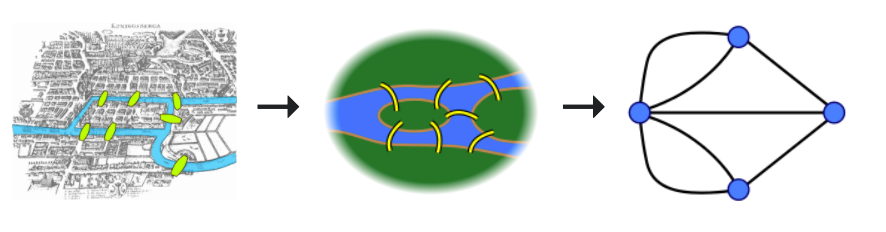
\includegraphics{./Figs/eiler.png}
\end{frame}

\begin{frame}{Rrjetet Gjeohapësinore}
\protect\hypertarget{rrjetet-gjeohapuxebsinore}{}
\begin{itemize}
\item
  Në shkencën e të dhënave gjeografike, rrjetet gjeohapësinore janë
  rrjete ku vendndodhja e nyjeve dhe skajeve është e nevojshme për t'i
  studiuar dhe përdorur për analizë.
\item
  Të tilla rrjete janë të kudogjendura dhe përfshijnë rrjetet e
  transportit, rrjetet hidrologjike, matricat origjinë-destinacion (të
  dhëna të rrjedhës), rrjetet e energjisë dhe rrjetet tregtare.
\end{itemize}
\end{frame}

\begin{frame}{Algoritmet e Rrjetit}
\protect\hypertarget{algoritmet-e-rrjetit}{}
\begin{itemize}
\item
  Një nga problemet themelore në grafe është llogaritja e rrugës më të
  shkurtër midis dy nyjeve.
\item
  Ky problem ka aplikime të panumërta në sektorin gjeohapësinor, duke
  përfshirë rrugëtimin nga pika A në B.
\end{itemize}
\end{frame}

\begin{frame}{Algoritmet e Rrjetit}
\protect\hypertarget{algoritmet-e-rrjetit-1}{}
\begin{itemize}
\tightlist
\item
  Që nga viti 1956, algoritmi i Dijkstra ka qenë mënyra më e famshme për
  të llogaritur një rrugë më të shkurtër në një graf me peshë.
\end{itemize}
\end{frame}

\begin{frame}[fragile]{Algoritmi i Dijkstra}
\protect\hypertarget{algoritmi-i-dijkstra}{}
\AddToHookNext{env/Highlighting/begin}{\tiny}

\begin{Shaded}
\begin{Highlighting}[]
\CommentTok{\#\# Prezantimi i Grafit dhe Nyjeve}

\ImportTok{import}\NormalTok{ networkx }\ImportTok{as}\NormalTok{ nx}
\ImportTok{import}\NormalTok{ matplotlib.pyplot }\ImportTok{as}\NormalTok{ plt}

\CommentTok{\# Krijoni graf{-}in}
\NormalTok{G }\OperatorTok{=}\NormalTok{ nx.Graph()}
\NormalTok{edges }\OperatorTok{=}\NormalTok{ [}
\NormalTok{    (}\StringTok{\textquotesingle{}A\textquotesingle{}}\NormalTok{, }\StringTok{\textquotesingle{}B\textquotesingle{}}\NormalTok{, }\DecValTok{1}\NormalTok{),}
\NormalTok{    (}\StringTok{\textquotesingle{}A\textquotesingle{}}\NormalTok{, }\StringTok{\textquotesingle{}C\textquotesingle{}}\NormalTok{, }\DecValTok{4}\NormalTok{),}
\NormalTok{    (}\StringTok{\textquotesingle{}B\textquotesingle{}}\NormalTok{, }\StringTok{\textquotesingle{}C\textquotesingle{}}\NormalTok{, }\DecValTok{2}\NormalTok{),}
\NormalTok{    (}\StringTok{\textquotesingle{}B\textquotesingle{}}\NormalTok{, }\StringTok{\textquotesingle{}D\textquotesingle{}}\NormalTok{, }\DecValTok{5}\NormalTok{),}
\NormalTok{    (}\StringTok{\textquotesingle{}C\textquotesingle{}}\NormalTok{, }\StringTok{\textquotesingle{}D\textquotesingle{}}\NormalTok{, }\DecValTok{1}\NormalTok{),}
\NormalTok{    (}\StringTok{\textquotesingle{}C\textquotesingle{}}\NormalTok{, }\StringTok{\textquotesingle{}E\textquotesingle{}}\NormalTok{, }\DecValTok{3}\NormalTok{),}
\NormalTok{    (}\StringTok{\textquotesingle{}D\textquotesingle{}}\NormalTok{, }\StringTok{\textquotesingle{}E\textquotesingle{}}\NormalTok{, }\DecValTok{2}\NormalTok{)}
\NormalTok{]}
\NormalTok{G.add\_weighted\_edges\_from(edges)}

\CommentTok{\# Vizualizoni graf{-}in}
\NormalTok{pos }\OperatorTok{=}\NormalTok{ nx.spring\_layout(G)}
\NormalTok{nx.draw(G, pos, with\_labels}\OperatorTok{=}\VariableTok{True}\NormalTok{, node\_color}\OperatorTok{=}\StringTok{\textquotesingle{}lightblue\textquotesingle{}}\NormalTok{, edge\_color}\OperatorTok{=}\StringTok{\textquotesingle{}grey\textquotesingle{}}\NormalTok{)}
\NormalTok{labels }\OperatorTok{=}\NormalTok{ nx.get\_edge\_attributes(G, }\StringTok{\textquotesingle{}weight\textquotesingle{}}\NormalTok{)}
\NormalTok{nx.draw\_networkx\_edge\_labels(G, pos, edge\_labels}\OperatorTok{=}\NormalTok{labels)}
\NormalTok{plt.show()}
\end{Highlighting}
\end{Shaded}
\end{frame}

\begin{frame}{Algoritmi i Dijkstra}
\protect\hypertarget{algoritmi-i-dijkstra-1}{}
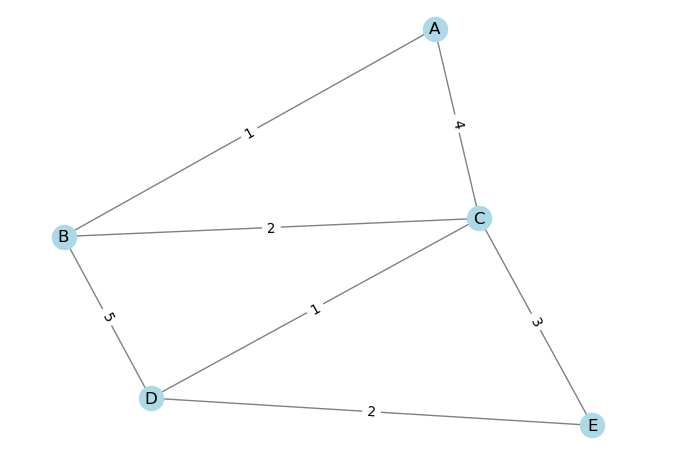
\includegraphics{./Figs/dijkstra1.png}
\end{frame}

\begin{frame}{Algoritmi i Dijkstra - Hapi 1}
\protect\hypertarget{algoritmi-i-dijkstra---hapi-1}{}
Filloni me nyjen fillestare (A)

\begin{itemize}
\tightlist
\item
  Distanca nga A në A: 0
\end{itemize}
\end{frame}

\begin{frame}{Algoritmi i Dijkstra - Hapi 2}
\protect\hypertarget{algoritmi-i-dijkstra---hapi-2}{}
Filloni me nyjen fillestare (A)

\begin{itemize}
\item
  Distanca nga A te fqinjët:

  B: 1

  C: 4
\item
  Rrugët më të shkurtra:

  A -\textgreater{} A: 0

  A -\textgreater{} B: 1

  A -\textgreater{} C: 4
\end{itemize}
\end{frame}

\begin{frame}{Algoritmi i Dijkstra - Hapi 3}
\protect\hypertarget{algoritmi-i-dijkstra---hapi-3}{}
Zgjidhni nyjen më të afërt (B)

\begin{itemize}
\item
  Distanca nga B te fqinjët:

  C: 3 (1 + 2)

  D: 6 (1 + 5)
\item
  Rrugët më të shkurtra:
\item
  A -\textgreater{} B: 1
\item
  A -\textgreater{} C: 3 (via B)
\item
  A -\textgreater{} D: 6 (via B)
\end{itemize}
\end{frame}

\begin{frame}{Algoritmi i Dijkstra - Hapi 4}
\protect\hypertarget{algoritmi-i-dijkstra---hapi-4}{}
Zgjidhni nyjen më të afërt të ardhshme (C)

\begin{itemize}
\item
  Distanca nga C te fqinjët:

  D: 4 (3 + 1)

  E: 6 (3 + 3)
\item
  Rrugët më të shkurtra:

  A -\textgreater{} B: 1

  A -\textgreater{} C: 3 (via B)

  A -\textgreater{} D: 4 (via C)

  A -\textgreater{} E: 6 (via C)
\end{itemize}
\end{frame}

\begin{frame}{Algoritmi i Dijkstra - Hapi 5}
\protect\hypertarget{algoritmi-i-dijkstra---hapi-5}{}
Zgjidhni nyjen më të afërt të ardhshme (D)

\begin{itemize}
\item
  Distanca nga D te fqinjët:

  E: 6 (via C)
\item
  Rrugët më të shkurtra:

  A -\textgreater{} B: 1

  A -\textgreater{} C: 3 (via B)

  A -\textgreater{} D: 4 (via C)

  A -\textgreater{} E: 6 (via C)
\end{itemize}

Distancat më të shkurtra janë: \{`A': (None, 0), `B': (`A', 1), `C':
(`B', 3), `D': (`C', 4), `E': (`C', 6)\} Rruga më e shkurtër nga A në E
është: {[}`A', `B', `C', `E'{]} me total 6.
\end{frame}

\begin{frame}[fragile]{Algoritmi i Dijkstra - Hapi 4}
\protect\hypertarget{algoritmi-i-dijkstra---hapi-4-1}{}
\AddToHookNext{env/Highlighting/begin}{\tiny}

\begin{Shaded}
\begin{Highlighting}[]
\ImportTok{import}\NormalTok{ networkx }\ImportTok{as}\NormalTok{ nx}

\CommentTok{\# Krijoni graf{-}in}
\NormalTok{G }\OperatorTok{=}\NormalTok{ nx.Graph()}
\NormalTok{edges }\OperatorTok{=}\NormalTok{ [}
\NormalTok{    (}\StringTok{\textquotesingle{}A\textquotesingle{}}\NormalTok{, }\StringTok{\textquotesingle{}B\textquotesingle{}}\NormalTok{, }\DecValTok{1}\NormalTok{),}
\NormalTok{    (}\StringTok{\textquotesingle{}A\textquotesingle{}}\NormalTok{, }\StringTok{\textquotesingle{}C\textquotesingle{}}\NormalTok{, }\DecValTok{4}\NormalTok{),}
\NormalTok{    (}\StringTok{\textquotesingle{}B\textquotesingle{}}\NormalTok{, }\StringTok{\textquotesingle{}C\textquotesingle{}}\NormalTok{, }\DecValTok{2}\NormalTok{),}
\NormalTok{    (}\StringTok{\textquotesingle{}B\textquotesingle{}}\NormalTok{, }\StringTok{\textquotesingle{}D\textquotesingle{}}\NormalTok{, }\DecValTok{5}\NormalTok{),}
\NormalTok{    (}\StringTok{\textquotesingle{}C\textquotesingle{}}\NormalTok{, }\StringTok{\textquotesingle{}D\textquotesingle{}}\NormalTok{, }\DecValTok{1}\NormalTok{),}
\NormalTok{    (}\StringTok{\textquotesingle{}C\textquotesingle{}}\NormalTok{, }\StringTok{\textquotesingle{}E\textquotesingle{}}\NormalTok{, }\DecValTok{3}\NormalTok{),}
\NormalTok{    (}\StringTok{\textquotesingle{}D\textquotesingle{}}\NormalTok{, }\StringTok{\textquotesingle{}E\textquotesingle{}}\NormalTok{, }\DecValTok{2}\NormalTok{)}
\NormalTok{]}
\NormalTok{G.add\_weighted\_edges\_from(edges)}

\CommentTok{\# Filloni me nyjen \textquotesingle{}A\textquotesingle{}}
\NormalTok{shortest\_paths }\OperatorTok{=}\NormalTok{ \{}\StringTok{\textquotesingle{}A\textquotesingle{}}\NormalTok{: (}\VariableTok{None}\NormalTok{, }\DecValTok{0}\NormalTok{)\}  }\CommentTok{\# Nyja \textquotesingle{}A\textquotesingle{} me kosto zero}
\NormalTok{current\_node }\OperatorTok{=} \StringTok{\textquotesingle{}A\textquotesingle{}}
\NormalTok{visited }\OperatorTok{=} \BuiltInTok{set}\NormalTok{()}

\CommentTok{\# Hapi 2 dhe 3: Zgjidhni nyjen më të afërt dhe llogaritni distancat}
\KeywordTok{def}\NormalTok{ calculate\_shortest\_paths(graph, start\_node):}
\NormalTok{    visited }\OperatorTok{=} \BuiltInTok{set}\NormalTok{()}
\NormalTok{    shortest\_paths }\OperatorTok{=}\NormalTok{ \{start\_node: (}\VariableTok{None}\NormalTok{, }\DecValTok{0}\NormalTok{)\}}
\NormalTok{    current\_node }\OperatorTok{=}\NormalTok{ start\_node}

    \ControlFlowTok{while}\NormalTok{ current\_node:}
\NormalTok{        visited.add(current\_node)}
\NormalTok{        destinations }\OperatorTok{=}\NormalTok{ graph[current\_node]}
\NormalTok{        weight\_to\_current\_node }\OperatorTok{=}\NormalTok{ shortest\_paths[current\_node][}\DecValTok{1}\NormalTok{]}
\end{Highlighting}
\end{Shaded}
\end{frame}

\begin{frame}[fragile]{Algoritmi i Dijkstra - Hapi 4}
\protect\hypertarget{algoritmi-i-dijkstra---hapi-4-2}{}
\AddToHookNext{env/Highlighting/begin}{\tiny}

\begin{Shaded}
\begin{Highlighting}[]
        \ControlFlowTok{for}\NormalTok{ next\_node, weight }\KeywordTok{in}\NormalTok{ destinations.items():}
\NormalTok{            weight }\OperatorTok{=}\NormalTok{ weight[}\StringTok{\textquotesingle{}weight\textquotesingle{}}\NormalTok{]}
\NormalTok{            total\_weight }\OperatorTok{=}\NormalTok{ weight\_to\_current\_node }\OperatorTok{+}\NormalTok{ weight}
            \ControlFlowTok{if}\NormalTok{ next\_node }\KeywordTok{not} \KeywordTok{in}\NormalTok{ shortest\_paths:}
\NormalTok{                shortest\_paths[next\_node] }\OperatorTok{=}\NormalTok{ (current\_node, total\_weight)}
            \ControlFlowTok{else}\NormalTok{:}
\NormalTok{                current\_weight }\OperatorTok{=}\NormalTok{ shortest\_paths[next\_node][}\DecValTok{1}\NormalTok{]}
                \ControlFlowTok{if}\NormalTok{ current\_weight }\OperatorTok{\textgreater{}}\NormalTok{ total\_weight:}
\NormalTok{                    shortest\_paths[next\_node] }\OperatorTok{=}\NormalTok{ (current\_node, total\_weight)}

\NormalTok{        next\_destinations }\OperatorTok{=}\NormalTok{ \{node: shortest\_paths[node] }\ControlFlowTok{for}\NormalTok{ node }\KeywordTok{in}\NormalTok{ shortest\_paths }\ControlFlowTok{if}\NormalTok{ node }\KeywordTok{not} \KeywordTok{in}\NormalTok{ visited\}}
        \ControlFlowTok{if} \KeywordTok{not}\NormalTok{ next\_destinations:}
            \ControlFlowTok{break}
\NormalTok{        current\_node }\OperatorTok{=} \BuiltInTok{min}\NormalTok{(next\_destinations, key}\OperatorTok{=}\KeywordTok{lambda}\NormalTok{ k: next\_destinations[k][}\DecValTok{1}\NormalTok{])}

    \ControlFlowTok{return}\NormalTok{ shortest\_paths}
\end{Highlighting}
\end{Shaded}
\end{frame}

\begin{frame}[fragile]{Algoritmi i Dijkstra - Hapi 4}
\protect\hypertarget{algoritmi-i-dijkstra---hapi-4-3}{}
\AddToHookNext{env/Highlighting/begin}{\tiny}

\begin{Shaded}
\begin{Highlighting}[]
\CommentTok{\# Llogaritni rrugët më të shkurtra nga \textquotesingle{}A\textquotesingle{} në të gjitha nyjet}
\NormalTok{shortest\_paths }\OperatorTok{=}\NormalTok{ calculate\_shortest\_paths(G, }\StringTok{\textquotesingle{}A\textquotesingle{}}\NormalTok{)}
\BuiltInTok{print}\NormalTok{(}\StringTok{"Distancat më të shkurtra janë:"}\NormalTok{, shortest\_paths)}

\CommentTok{\# Për rrugën më të shkurtër nga A në E}
\KeywordTok{def}\NormalTok{ get\_path(shortest\_paths, end\_node):}
\NormalTok{    path }\OperatorTok{=}\NormalTok{ []}
    \ControlFlowTok{while}\NormalTok{ end\_node:}
\NormalTok{        path.append(end\_node)}
\NormalTok{        next\_node }\OperatorTok{=}\NormalTok{ shortest\_paths[end\_node][}\DecValTok{0}\NormalTok{]}
\NormalTok{        end\_node }\OperatorTok{=}\NormalTok{ next\_node}
\NormalTok{    path }\OperatorTok{=}\NormalTok{ path[::}\OperatorTok{{-}}\DecValTok{1}\NormalTok{]}
    \ControlFlowTok{return}\NormalTok{ path}

\CommentTok{\# Gjeni rrugën më të shkurtër nga A në E}
\NormalTok{shortest\_path }\OperatorTok{=}\NormalTok{ get\_path(shortest\_paths, }\StringTok{\textquotesingle{}E\textquotesingle{}}\NormalTok{)}
\BuiltInTok{print}\NormalTok{(}\StringTok{"Rruga më e shkurtër nga A në E është:"}\NormalTok{, shortest\_path)}
\end{Highlighting}
\end{Shaded}
\end{frame}

\begin{frame}{Krijimi i Grafit}
\protect\hypertarget{krijimi-i-grafit}{}
\begin{itemize}
\item
  Le të krijojmë një graf me skaje të peshësuara.
\item
  Peshat mund të përfaqësojnë për shembull koston e përshkimit të një
  skaji (p.sh., një skaj i gjatë ka një peshë më të madhe se një i
  shkurtër) dhe përdoren shumë shpesh për të përfaqësuar sisteme.
\end{itemize}
\end{frame}

\begin{frame}[fragile]{Krijimi i Grafit}
\protect\hypertarget{krijimi-i-grafit-1}{}
Në disa skenarë, grafet mund të krijohen dhe popullohen drejtpërdrejt me
networkx:

\AddToHookNext{env/Highlighting/begin}{\tiny}

\begin{Shaded}
\begin{Highlighting}[]
\ImportTok{import}\NormalTok{ networkx }\ImportTok{as}\NormalTok{ nx}
\ImportTok{import}\NormalTok{ matplotlib.pyplot }\ImportTok{as}\NormalTok{ plt}

\CommentTok{\# krijoni një graf të thjeshtë të pa drejtuar}
\NormalTok{g }\OperatorTok{=}\NormalTok{ nx.Graph(name}\OperatorTok{=}\StringTok{\textquotesingle{}graf i vogël\textquotesingle{}}\NormalTok{)}

\CommentTok{\# shtoni skaje me një atribut (peshë)}
\NormalTok{g.add\_edge(}\StringTok{\textquotesingle{}a\textquotesingle{}}\NormalTok{, }\StringTok{\textquotesingle{}b\textquotesingle{}}\NormalTok{, weight}\OperatorTok{=}\FloatTok{0.1}\NormalTok{)}
\NormalTok{g.add\_edge(}\StringTok{\textquotesingle{}b\textquotesingle{}}\NormalTok{, }\StringTok{\textquotesingle{}c\textquotesingle{}}\NormalTok{, weight}\OperatorTok{=}\FloatTok{1.5}\NormalTok{)}
\NormalTok{g.add\_edge(}\StringTok{\textquotesingle{}a\textquotesingle{}}\NormalTok{, }\StringTok{\textquotesingle{}c\textquotesingle{}}\NormalTok{, weight}\OperatorTok{=}\FloatTok{1.0}\NormalTok{)}
\NormalTok{g.add\_edge(}\StringTok{\textquotesingle{}c\textquotesingle{}}\NormalTok{, }\StringTok{\textquotesingle{}d\textquotesingle{}}\NormalTok{, weight}\OperatorTok{=}\FloatTok{2.2}\NormalTok{)}

\CommentTok{\# Printoni informacionin e grafit}
\BuiltInTok{print}\NormalTok{(}\StringTok{"Emri:"}\NormalTok{, g.graph[}\StringTok{\textquotesingle{}name\textquotesingle{}}\NormalTok{])}
\BuiltInTok{print}\NormalTok{(}\StringTok{"Tipi:"}\NormalTok{, }\BuiltInTok{type}\NormalTok{(g))}
\BuiltInTok{print}\NormalTok{(}\StringTok{"Numri i nyjeve:"}\NormalTok{, g.number\_of\_nodes())}
\BuiltInTok{print}\NormalTok{(}\StringTok{"Numri i skajeve:"}\NormalTok{, g.number\_of\_edges())}
\BuiltInTok{print}\NormalTok{(}\StringTok{"Shkalla mesatare:"}\NormalTok{, }\BuiltInTok{sum}\NormalTok{(}\BuiltInTok{dict}\NormalTok{(g.degree()).values()) }\OperatorTok{/}\NormalTok{ g.number\_of\_nodes())}
\end{Highlighting}
\end{Shaded}
\end{frame}

\begin{frame}{Vizualizimi i Grafit}
\protect\hypertarget{vizualizimi-i-grafit}{}
\begin{itemize}
\item
  Veçanërisht për rrjete të vogla, është e mundur t'i vizatojmë ato
  drejtpërdrejt.
\item
  Vini re se ky graf i pa drejtuar është jo-hapësinor, në kuptimin që
  nyjet nuk kanë një vendndodhje të caktuar hapësinore.
\end{itemize}
\end{frame}

\begin{frame}[fragile]{Vizualizimi i Grafit}
\protect\hypertarget{vizualizimi-i-grafit-1}{}
\AddToHookNext{env/Highlighting/begin}{\tiny}

\begin{Shaded}
\begin{Highlighting}[]
\CommentTok{\# gjeneroni pozicionet e nyjeve duke përdorur një paraqitje të njohur}
\NormalTok{pos }\OperatorTok{=}\NormalTok{ nx.spring\_layout(g)}

\CommentTok{\# hapni vizatimin}
\NormalTok{nx.draw\_networkx(g, pos}\OperatorTok{=}\NormalTok{pos, font\_color}\OperatorTok{=}\StringTok{\textquotesingle{}white\textquotesingle{}}\NormalTok{)}

\CommentTok{\# vizatoni etiketat e skajeve}
\NormalTok{nx.draw\_networkx\_edge\_labels(g, pos}\OperatorTok{=}\NormalTok{pos)}

\CommentTok{\# vizatoni skajet}
\NormalTok{nx.draw\_networkx\_edges(g, pos}\OperatorTok{=}\NormalTok{pos)}

\CommentTok{\# shfaqni graf{-}in}
\NormalTok{plt.show()}
\end{Highlighting}
\end{Shaded}
\end{frame}

\begin{frame}[fragile]{Aksesimi i Elementeve të Grafit}
\protect\hypertarget{aksesimi-i-elementeve-tuxeb-grafit}{}
\begin{itemize}
\tightlist
\item
  Elementet e grafit mund të aksesohen drejtpërdrejt
\end{itemize}

\AddToHookNext{env/Highlighting/begin}{\tiny}

\begin{Shaded}
\begin{Highlighting}[]
\CommentTok{\# Nyjet e grafit}
\NormalTok{g.nodes}
\CommentTok{\# NodeView((\textquotesingle{}a\textquotesingle{}, \textquotesingle{}b\textquotesingle{}, \textquotesingle{}c\textquotesingle{}, \textquotesingle{}d\textquotesingle{}))}

\CommentTok{\# Skajet e grafit}
\NormalTok{g.edges}
\CommentTok{\# EdgeView([(\textquotesingle{}a\textquotesingle{}, \textquotesingle{}b\textquotesingle{}), (\textquotesingle{}a\textquotesingle{}, \textquotesingle{}c\textquotesingle{}), (\textquotesingle{}b\textquotesingle{}, \textquotesingle{}c\textquotesingle{}), (\textquotesingle{}c\textquotesingle{}, \textquotesingle{}d\textquotesingle{})])}
\end{Highlighting}
\end{Shaded}
\end{frame}

\begin{frame}[fragile]{Aksesimi i Elementeve të Grafit}
\protect\hypertarget{aksesimi-i-elementeve-tuxeb-grafit-1}{}
\AddToHookNext{env/Highlighting/begin}{\tiny}

\begin{Shaded}
\begin{Highlighting}[]
\CommentTok{\# shikoni nyjet fqinje të nyjës \textquotesingle{}a\textquotesingle{}:}
\ControlFlowTok{for}\NormalTok{ node\_nei }\KeywordTok{in}\NormalTok{ g.neighbors(}\StringTok{\textquotesingle{}a\textquotesingle{}}\NormalTok{):}
    \BuiltInTok{print}\NormalTok{(node\_nei)}
\end{Highlighting}
\end{Shaded}
\end{frame}

\begin{frame}[fragile]{Aksesimi i Atributeve}
\protect\hypertarget{aksesimi-i-atributeve}{}
\AddToHookNext{env/Highlighting/begin}{\tiny}

\begin{Shaded}
\begin{Highlighting}[]
\NormalTok{weights }\OperatorTok{=}\NormalTok{ nx.get\_edge\_attributes(g, }\StringTok{\textquotesingle{}weight\textquotesingle{}}\NormalTok{)}
\NormalTok{weights}
\CommentTok{\# \{(\textquotesingle{}a\textquotesingle{}, \textquotesingle{}b\textquotesingle{}): 0.1, (\textquotesingle{}a\textquotesingle{}, \textquotesingle{}c\textquotesingle{}): 1.0, (\textquotesingle{}b\textquotesingle{}, \textquotesingle{}c\textquotesingle{}): 1.5, (\textquotesingle{}c\textquotesingle{}, \textquotesingle{}d\textquotesingle{}): 2.2\}}
\end{Highlighting}
\end{Shaded}
\end{frame}

\begin{frame}{Llogaritja e Rrugës më të Shkurtër}
\protect\hypertarget{llogaritja-e-rruguxebs-muxeb-tuxeb-shkurtuxebr}{}
\begin{itemize}
\item
  Tani mund të përdorim \textbf{networkx} për të llogaritur rrugën më të
  shkurtër midis nyjeve.
\item
  Fillimisht, mund të llogarisim rrugën më të shkurtër të peshuar
  (\textbf{unweighted shortest path}), duke supozuar se të gjitha skajet
  kanë të njëjtën peshë:
\end{itemize}
\end{frame}

\begin{frame}[fragile]{Llogaritja e Rrugës më të Shkurtër}
\protect\hypertarget{llogaritja-e-rruguxebs-muxeb-tuxeb-shkurtuxebr-1}{}
\AddToHookNext{env/Highlighting/begin}{\tiny}

\begin{Shaded}
\begin{Highlighting}[]
\NormalTok{unweighted\_path }\OperatorTok{=}\NormalTok{ nx.shortest\_path(g, }\StringTok{\textquotesingle{}b\textquotesingle{}}\NormalTok{, }\StringTok{\textquotesingle{}d\textquotesingle{}}\NormalTok{)}
\NormalTok{unweighted\_path}
\end{Highlighting}
\end{Shaded}
\end{frame}

\begin{frame}{Rruga e Peshuar}
\protect\hypertarget{rruga-e-peshuar}{}
\begin{itemize}
\tightlist
\item
  Tani, mund të shohim rrugën më të shkurtër të peshuar
  (\textbf{weighted shortest path}), duke vënë re se shuma e peshave të
  \textbf{(bacd)} është më e lehtë se \textbf{(bcd)}:
\end{itemize}
\end{frame}

\begin{frame}[fragile]{Rruga e Peshua}
\protect\hypertarget{rruga-e-peshua}{}
\AddToHookNext{env/Highlighting/begin}{\tiny}

\begin{Shaded}
\begin{Highlighting}[]
\NormalTok{weighted\_path }\OperatorTok{=}\NormalTok{ nx.shortest\_path(g, }\StringTok{\textquotesingle{}b\textquotesingle{}}\NormalTok{, }\StringTok{\textquotesingle{}d\textquotesingle{}}\NormalTok{, weight}\OperatorTok{=}\StringTok{\textquotesingle{}weight\textquotesingle{}}\NormalTok{)}
\NormalTok{weighted\_path}
\end{Highlighting}
\end{Shaded}
\end{frame}

\begin{frame}{Metrikat e Rrjetit}
\protect\hypertarget{metrikat-e-rrjetit}{}
\begin{itemize}
\item
  Për të përshkruar dhe kuptuar rrjetet, janë krijuar shumë metrika.
\item
  Për shembull, ne mund të shohim se sa skaje janë të lidhura me një
  nyje (shkalla (\textbf{degree }) e një nyje).
\end{itemize}
\end{frame}

\begin{frame}{Metrikat e Rrjetit}
\protect\hypertarget{metrikat-e-rrjetit-1}{}
\begin{itemize}
\item
  Nyja `a' ka dy skaje, ndërsa `c' ka 3.
\item
  Disa nyje me shkallë të lartë janë ``qendra'', duke lidhur shumë nyje:
  Për shembull, në rrjetet sociale, politikanët janë qendra.
\end{itemize}
\end{frame}

\begin{frame}{Metrikat e Rrjetit}
\protect\hypertarget{metrikat-e-rrjetit-2}{}
\begin{itemize}
\tightlist
\item
  Qendra (\textbf{centrality}) i një nyje është gjithashtu i
  rëndësishëm: Sa ``hapje'' në skaje janë të nevojshme për të arritur të
  gjitha nyjet e tjera?
\end{itemize}
\end{frame}

\begin{frame}{Metrikat e Rrjetit}
\protect\hypertarget{metrikat-e-rrjetit-3}{}
\begin{itemize}
\tightlist
\item
  Për shembull, Londra është një qendër e udhëtimeve ajrore më e
  rëndësishme se çdo qytet tjetër në Mbretërinë e Bashkuar
\end{itemize}
\end{frame}

\begin{frame}[fragile]{Metrikat e Rrjetit}
\protect\hypertarget{metrikat-e-rrjetit-4}{}
\AddToHookNext{env/Highlighting/begin}{\tiny}

\begin{Shaded}
\begin{Highlighting}[]
\ImportTok{import}\NormalTok{ networkx }\ImportTok{as}\NormalTok{ nx}

\CommentTok{\# Krijo graf{-}in}
\NormalTok{g }\OperatorTok{=}\NormalTok{ nx.Graph(name}\OperatorTok{=}\StringTok{\textquotesingle{}graf i vogël\textquotesingle{}}\NormalTok{)}
\NormalTok{g.add\_edge(}\StringTok{\textquotesingle{}a\textquotesingle{}}\NormalTok{, }\StringTok{\textquotesingle{}b\textquotesingle{}}\NormalTok{, weight}\OperatorTok{=}\FloatTok{0.1}\NormalTok{)}
\NormalTok{g.add\_edge(}\StringTok{\textquotesingle{}b\textquotesingle{}}\NormalTok{, }\StringTok{\textquotesingle{}c\textquotesingle{}}\NormalTok{, weight}\OperatorTok{=}\FloatTok{1.5}\NormalTok{)}
\NormalTok{g.add\_edge(}\StringTok{\textquotesingle{}a\textquotesingle{}}\NormalTok{, }\StringTok{\textquotesingle{}c\textquotesingle{}}\NormalTok{, weight}\OperatorTok{=}\FloatTok{1.0}\NormalTok{)}
\NormalTok{g.add\_edge(}\StringTok{\textquotesingle{}c\textquotesingle{}}\NormalTok{, }\StringTok{\textquotesingle{}d\textquotesingle{}}\NormalTok{, weight}\OperatorTok{=}\FloatTok{2.2}\NormalTok{)}

\CommentTok{\# Ekstraktoni të gjitha shkallët: kjo është zakonisht një pjesë e rëndësishme e informacionit për të kuptuar strukturën e grafit.}
\NormalTok{g.degree()}
\end{Highlighting}
\end{Shaded}
\end{frame}

\begin{frame}[fragile]{Metrikat e Rrjetit}
\protect\hypertarget{metrikat-e-rrjetit-5}{}
\AddToHookNext{env/Highlighting/begin}{\tiny}

\begin{Shaded}
\begin{Highlighting}[]
\CommentTok{\# Nxirrni shkallët në një listë të thjeshtë}
\NormalTok{degrees }\OperatorTok{=}\NormalTok{ [deg }\ControlFlowTok{for}\NormalTok{ node, deg }\KeywordTok{in}\NormalTok{ g.degree()]}
\NormalTok{degrees}
\end{Highlighting}
\end{Shaded}
\end{frame}

\begin{frame}[fragile]{Metrikat e Rrjetit}
\protect\hypertarget{metrikat-e-rrjetit-6}{}
\AddToHookNext{env/Highlighting/begin}{\tiny}

\begin{Shaded}
\begin{Highlighting}[]
\CommentTok{\# \textquotesingle{}c\textquotesingle{} është nyja më qendrore, pasi mund të arrijmë të gjitha nyjet e tjera me numrin më të vogël të hapave, ndërsa \textquotesingle{}d\textquotesingle{} është nyja më e izoluar.}
\NormalTok{nx.algorithms.centrality.degree\_centrality(g)}
\end{Highlighting}
\end{Shaded}
\end{frame}

\begin{frame}{Centraliteti dhe Pesha}
\protect\hypertarget{centraliteti-dhe-pesha}{}
\begin{itemize}
\tightlist
\item
  Një tjetër metrikë popullore e qendralitetit është \textbf{betweeness
  centrality} i bazuar në rrugët më të shkurtra midis nyjeve
\end{itemize}
\end{frame}

\begin{frame}{Centraliteti dhe Pesha}
\protect\hypertarget{centraliteti-dhe-pesha-1}{}
\begin{itemize}
\tightlist
\item
  Peshat e skajeve \textbf{Edge weights} mund të jenë të rëndësishme për
  të llogaritur centralitetin dhe metrika të tjera.
\end{itemize}
\end{frame}

\begin{frame}[fragile]{Metrikat e Rrjetit}
\protect\hypertarget{metrikat-e-rrjetit-7}{}
\AddToHookNext{env/Highlighting/begin}{\tiny}

\begin{Shaded}
\begin{Highlighting}[]
\CommentTok{\# Centraliteti i nyjeve}
\NormalTok{nx.algorithms.centrality.betweenness\_centrality(g, weight}\OperatorTok{=}\StringTok{\textquotesingle{}weight\textquotesingle{}}\NormalTok{)}
\CommentTok{\# \textquotesingle{}a\textquotesingle{} dhe \textquotesingle{}b\textquotesingle{} janë nyjet më qendrore të grafit}
\end{Highlighting}
\end{Shaded}
\end{frame}

\begin{frame}[fragile]{Metrikat e Rrjetit}
\protect\hypertarget{metrikat-e-rrjetit-8}{}
\AddToHookNext{env/Highlighting/begin}{\tiny}

\begin{Shaded}
\begin{Highlighting}[]
\CommentTok{\# Centraliteti i skajeve}
\NormalTok{nx.algorithms.centrality.edge\_betweenness\_centrality(g, weight}\OperatorTok{=}\StringTok{\textquotesingle{}weight\textquotesingle{}}\NormalTok{)}
\CommentTok{\# \textquotesingle{}ac\textquotesingle{} është skaji më qendror i grafit}
\end{Highlighting}
\end{Shaded}
\end{frame}

\begin{frame}{Rrjetet Tregtare}
\protect\hypertarget{rrjetet-tregtare}{}
\begin{itemize}
\item
  Analiza e rrjetave aplikohet me sukses për të modeluar ndërveprimet në
  ekonomi, sociologji dhe fusha të tjera.
\item
  Të dhënat nga kjo analizë përfaqësojnë ndërveprimet tregtare midis
  palëve (p.sh. tregtia e kafshëve midis Argjentinës dhe Brazilit në
  vitin 2017).
\end{itemize}
\end{frame}

\begin{frame}[fragile]{Rrjetet Tregtare}
\protect\hypertarget{rrjetet-tregtare-1}{}
Rrjetet e marra nga këto të dhëna do të ofrojnë një pamje të anuar mbi
tregtinë botërore.

\AddToHookNext{env/Highlighting/begin}{\tiny}

\begin{Shaded}
\begin{Highlighting}[]
\ImportTok{import}\NormalTok{ pandas }\ImportTok{as}\NormalTok{ pd}

\CommentTok{\# ngarkoni të dhënat nga një skedar TSV duke përdorur pandas}
\NormalTok{trade\_df }\OperatorTok{=}\NormalTok{ pd.read\_csv(}\StringTok{\textquotesingle{}data/gis4/trade\_network\_wits{-}1988\_2018.tsv\textquotesingle{}}\NormalTok{, sep}\OperatorTok{=}\StringTok{\textquotesingle{}}\CharTok{\textbackslash{}t}\StringTok{\textquotesingle{}}\NormalTok{)}
\CommentTok{\# shfaqni katër rreshta shembuj nga të dhënat e ngarkuara}
\NormalTok{trade\_df.sample(}\DecValTok{4}\NormalTok{)}
\end{Highlighting}
\end{Shaded}
\end{frame}

\begin{frame}{Rrjetet Tregtare}
\protect\hypertarget{rrjetet-tregtare-2}{}
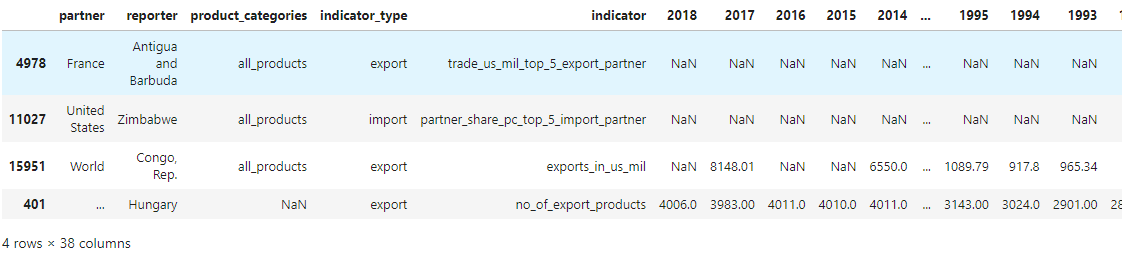
\includegraphics{./Figs/trade1.png}
\end{frame}

\begin{frame}{Rrjetet Tregtare}
\protect\hypertarget{rrjetet-tregtare-3}{}
Pasi kemi ngarkuar dhe shfaqur disa rreshta shembull nga të dhënat, le
të përqendrohemi në të dhënat e vitit 2018 dhe të heqim të dhënat e
paplota:
\end{frame}

\begin{frame}[fragile]{Rrjetet Tregtare}
\protect\hypertarget{rrjetet-tregtare-4}{}
\AddToHookNext{env/Highlighting/begin}{\tiny}

\begin{Shaded}
\begin{Highlighting}[]
\ImportTok{import}\NormalTok{ pandas }\ImportTok{as}\NormalTok{ pd}
\CommentTok{\# përzgjedhja e kolonave të interesit për analizë}
\NormalTok{trade\_df }\OperatorTok{=}\NormalTok{ trade\_df[[}\StringTok{\textquotesingle{}reporter\_country\_code\textquotesingle{}}\NormalTok{,}\StringTok{\textquotesingle{}reporter\textquotesingle{}}\NormalTok{,}\StringTok{\textquotesingle{}partner\_country\_code\textquotesingle{}}\NormalTok{,}\StringTok{\textquotesingle{}partner\textquotesingle{}}\NormalTok{,}
                     \StringTok{\textquotesingle{}product\_categories\textquotesingle{}}\NormalTok{,}\StringTok{\textquotesingle{}indicator\_type\textquotesingle{}}\NormalTok{,}\StringTok{\textquotesingle{}indicator\textquotesingle{}}\NormalTok{,}\StringTok{\textquotesingle{}2018\textquotesingle{}}\NormalTok{]]}

\CommentTok{\# përqendrimi në vëllimin total në USD të importit/eksportit midis vendeve}
\NormalTok{trade\_df }\OperatorTok{=}\NormalTok{ trade\_df[}\OperatorTok{\textasciitilde{}}\NormalTok{trade\_df[}\StringTok{\textquotesingle{}reporter\_country\_code\textquotesingle{}}\NormalTok{].isnull()]}
\NormalTok{trade\_df }\OperatorTok{=}\NormalTok{ trade\_df[}\OperatorTok{\textasciitilde{}}\NormalTok{trade\_df[}\StringTok{\textquotesingle{}partner\_country\_code\textquotesingle{}}\NormalTok{].isnull()]}
\CommentTok{\# heqja e të dhënave të paplota}
\NormalTok{trade\_df }\OperatorTok{=}\NormalTok{ trade\_df[}\OperatorTok{\textasciitilde{}}\NormalTok{trade\_df[}\StringTok{\textquotesingle{}2018\textquotesingle{}}\NormalTok{].isnull()]}
\NormalTok{trade\_df }\OperatorTok{=}\NormalTok{ trade\_df[trade\_df[}\StringTok{\textquotesingle{}product\_categories\textquotesingle{}}\NormalTok{]}\OperatorTok{==}\StringTok{\textquotesingle{}all\_products\textquotesingle{}}\NormalTok{]}

\CommentTok{\# përqendrimi në tregtarët më të mëdhenj të importit/eksportit}
\NormalTok{trade\_df }\OperatorTok{=}\NormalTok{ trade\_df[trade\_df[}\StringTok{\textquotesingle{}indicator\textquotesingle{}}\NormalTok{].isin([}\StringTok{\textquotesingle{}partner\_share\_pc\_top\_5\_import\_partner\textquotesingle{}}\NormalTok{,}\StringTok{\textquotesingle{}partner\_share\_pc\_top\_5\_export\_partner\textquotesingle{}}\NormalTok{])]}
\CommentTok{\# kolonat e tjera interesante janë: \textquotesingle{}trade\_us\_mil\_top\_5\_export\_partner\textquotesingle{},\textquotesingle{}trade\_us\_mil\_top\_5\_import\_partner\textquotesingle{}}
\end{Highlighting}
\end{Shaded}
\end{frame}

\begin{frame}[fragile]{Rrjetet Tregtare}
\protect\hypertarget{rrjetet-tregtare-5}{}
\AddToHookNext{env/Highlighting/begin}{\tiny}

\begin{Shaded}
\begin{Highlighting}[]
\CommentTok{\# numri total i rreshtave të filtruar}
\BuiltInTok{len}\NormalTok{(trade\_df)}
\end{Highlighting}
\end{Shaded}
\end{frame}

\begin{frame}[fragile]{Rrjetet Tregtare}
\protect\hypertarget{rrjetet-tregtare-6}{}
Për të parë shembullin e rrjetit tregtar të Kinës:

\AddToHookNext{env/Highlighting/begin}{\tiny}

\begin{Shaded}
\begin{Highlighting}[]
\CommentTok{\# shembull i rrjetit tregtar të Kinës}
\NormalTok{trade\_df[trade\_df.reporter\_country\_code}\OperatorTok{==}\StringTok{\textquotesingle{}CHN\textquotesingle{}}\NormalTok{]}
\end{Highlighting}
\end{Shaded}
\end{frame}

\begin{frame}{Rrjetet Tregtare}
\protect\hypertarget{rrjetet-tregtare-7}{}
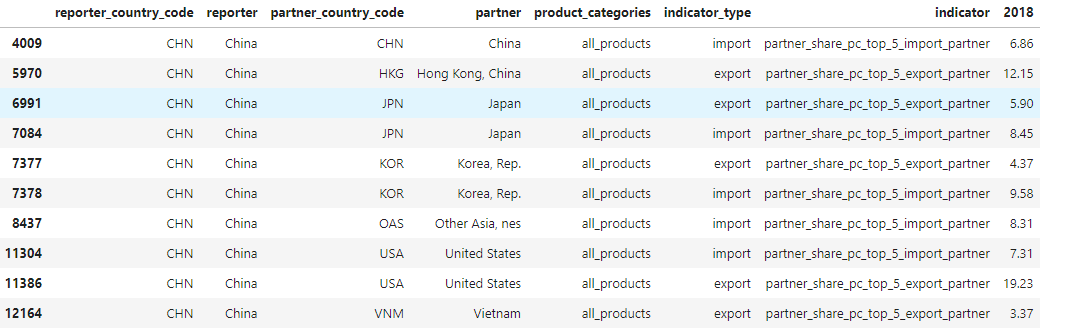
\includegraphics{./Figs/trade2.png}
\end{frame}

\begin{frame}[fragile]{Grafet nga dataframe}
\protect\hypertarget{grafet-nga-dataframe}{}
\AddToHookNext{env/Highlighting/begin}{\tiny}

\begin{Shaded}
\begin{Highlighting}[]
\ImportTok{import}\NormalTok{ networkx }\ImportTok{as}\NormalTok{ nx}
\ImportTok{import}\NormalTok{ matplotlib.pyplot }\ImportTok{as}\NormalTok{ plt}

\CommentTok{\# Define a function to print graph information manually}
\KeywordTok{def}\NormalTok{ print\_graph\_info(g):}
\NormalTok{    num\_nodes }\OperatorTok{=}\NormalTok{ g.number\_of\_nodes()}
\NormalTok{    num\_edges }\OperatorTok{=}\NormalTok{ g.number\_of\_edges()}
\NormalTok{    avg\_in\_degree }\OperatorTok{=} \BuiltInTok{sum}\NormalTok{(}\BuiltInTok{dict}\NormalTok{(g.in\_degree()).values()) }\OperatorTok{/}\NormalTok{ num\_nodes}
\NormalTok{    avg\_out\_degree }\OperatorTok{=} \BuiltInTok{sum}\NormalTok{(}\BuiltInTok{dict}\NormalTok{(g.out\_degree()).values()) }\OperatorTok{/}\NormalTok{ num\_nodes}

    \BuiltInTok{print}\NormalTok{(}\SpecialStringTok{f"Emri:"}\NormalTok{)}
    \BuiltInTok{print}\NormalTok{(}\SpecialStringTok{f"Tipi: }\SpecialCharTok{\{}\BuiltInTok{type}\NormalTok{(g)}\SpecialCharTok{.}\VariableTok{\_\_name\_\_}\SpecialCharTok{\}}\SpecialStringTok{"}\NormalTok{)}
    \BuiltInTok{print}\NormalTok{(}\SpecialStringTok{f"Numri i nyjeve: }\SpecialCharTok{\{}\NormalTok{num\_nodes}\SpecialCharTok{\}}\SpecialStringTok{"}\NormalTok{)}
    \BuiltInTok{print}\NormalTok{(}\SpecialStringTok{f"Numri i degeve: }\SpecialCharTok{\{}\NormalTok{num\_edges}\SpecialCharTok{\}}\SpecialStringTok{"}\NormalTok{)}
    \BuiltInTok{print}\NormalTok{(}\SpecialStringTok{f"Mesatarja brenda në gradë: }\SpecialCharTok{\{}\NormalTok{avg\_in\_degree}\SpecialCharTok{:.4f\}}\SpecialStringTok{"}\NormalTok{)}
    \BuiltInTok{print}\NormalTok{(}\SpecialStringTok{f"Mesatarja jashtë në gradë: }\SpecialCharTok{\{}\NormalTok{avg\_out\_degree}\SpecialCharTok{:.4f\}}\SpecialStringTok{"}\NormalTok{)}

\CommentTok{\# Gjeneroni grafikun nga data frame (lista e degeve)}
\NormalTok{df }\OperatorTok{=}\NormalTok{ trade\_df[trade\_df.indicator }\OperatorTok{==} \StringTok{\textquotesingle{}partner\_share\_pc\_top\_5\_import\_partner\textquotesingle{}}\NormalTok{]}
\NormalTok{trade\_import\_g }\OperatorTok{=}\NormalTok{ nx.from\_pandas\_edgelist(df, }\StringTok{\textquotesingle{}reporter\textquotesingle{}}\NormalTok{, }\StringTok{\textquotesingle{}partner\textquotesingle{}}\NormalTok{, [}\StringTok{\textquotesingle{}2018\textquotesingle{}}\NormalTok{], create\_using}\OperatorTok{=}\NormalTok{nx.DiGraph())}
\NormalTok{print\_graph\_info(trade\_import\_g)}
\end{Highlighting}
\end{Shaded}
\end{frame}

\begin{frame}{Grafet nga dataframe}
\protect\hypertarget{grafet-nga-dataframe-1}{}
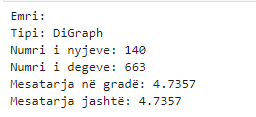
\includegraphics{./Figs/trade3.png}
\end{frame}

\begin{frame}[fragile]{Grafet nga dataframe}
\protect\hypertarget{grafet-nga-dataframe-2}{}
\AddToHookNext{env/Highlighting/begin}{\tiny}

\begin{Shaded}
\begin{Highlighting}[]
\CommentTok{\# Gjeneroni grafikun nga data frame  (lista e skajeve)}
\NormalTok{df }\OperatorTok{=}\NormalTok{ trade\_df[trade\_df.indicator}\OperatorTok{==}\StringTok{\textquotesingle{}partner\_share\_pc\_top\_5\_export\_partner\textquotesingle{}}\NormalTok{]}
\NormalTok{trade\_export\_g }\OperatorTok{=}\NormalTok{ nx.from\_pandas\_edgelist(df, }\StringTok{\textquotesingle{}reporter\textquotesingle{}}\NormalTok{, }\StringTok{\textquotesingle{}partner\textquotesingle{}}\NormalTok{, [}\StringTok{\textquotesingle{}2018\textquotesingle{}}\NormalTok{], create\_using}\OperatorTok{=}\NormalTok{nx.DiGraph())}
\NormalTok{print\_graph\_info(trade\_export\_g)}
\end{Highlighting}
\end{Shaded}
\end{frame}

\begin{frame}{Grafet nga dataframe}
\protect\hypertarget{grafet-nga-dataframe-3}{}
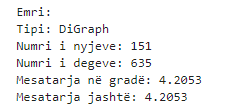
\includegraphics{./Figs/trade4.png}
\end{frame}

\begin{frame}[fragile]{Shkalla e plot in- and out}
\protect\hypertarget{shkalla-e-plot-in--and-out}{}
Hapi i parë për të kuptuar strukturën e një rrjeti është llogaritja e
shkallës së çdo nyje (numri i skajeve).

\AddToHookNext{env/Highlighting/begin}{\tiny}

\begin{Shaded}
\begin{Highlighting}[]
\KeywordTok{def}\NormalTok{ plot\_graph\_degrees(g, title, logscale}\OperatorTok{=}\VariableTok{False}\NormalTok{):}
    \CommentTok{"""}
\CommentTok{    Paraqitni shkallën e hyrjes dhe daljes së grafikut g në një grafik linje.}
\CommentTok{    @ g: një grafik}
\CommentTok{    @ title: titulli i grafikës}
\CommentTok{    @ logscale: transformoni boshtet x dhe y me log10}
\CommentTok{    """}
    \CommentTok{\# merrni shkallët}
\NormalTok{    indegrees }\OperatorTok{=}\NormalTok{ [deg }\ControlFlowTok{for}\NormalTok{ node, deg }\KeywordTok{in}\NormalTok{ g.in\_degree()]}
\NormalTok{    outdegrees }\OperatorTok{=}\NormalTok{ [deg }\ControlFlowTok{for}\NormalTok{ node, deg }\KeywordTok{in}\NormalTok{ g.out\_degree()]}
    \CommentTok{\# numërimi i shkallës në hyrje}
\NormalTok{    indeg\_vals }\OperatorTok{=} \BuiltInTok{sorted}\NormalTok{(}\BuiltInTok{list}\NormalTok{(}\BuiltInTok{set}\NormalTok{(indegrees)))}
\NormalTok{    indeg\_hist }\OperatorTok{=}\NormalTok{ [indegrees.count(x) }\ControlFlowTok{for}\NormalTok{ x }\KeywordTok{in}\NormalTok{ indeg\_vals]}
    \CommentTok{\# numërimi i shkallës në dalje}
\NormalTok{    outdeg\_vals }\OperatorTok{=} \BuiltInTok{sorted}\NormalTok{(}\BuiltInTok{list}\NormalTok{(}\BuiltInTok{set}\NormalTok{(outdegrees)))}
\NormalTok{    outdeg\_hist }\OperatorTok{=}\NormalTok{ [outdegrees.count(x) }\ControlFlowTok{for}\NormalTok{ x }\KeywordTok{in}\NormalTok{ outdeg\_vals]}
    \CommentTok{\# shtoni informacionin në titull}
\NormalTok{    title }\OperatorTok{=}\NormalTok{ title }\OperatorTok{+} \StringTok{" ["} \OperatorTok{+} \BuiltInTok{str}\NormalTok{(}\BuiltInTok{len}\NormalTok{(g.nodes)) }\OperatorTok{+} \StringTok{" nyje, "} \OperatorTok{+} \BuiltInTok{str}\NormalTok{(}\BuiltInTok{len}\NormalTok{(g.edges)) }\OperatorTok{+} \StringTok{" skaje]"}
    \CommentTok{\# paraqitni}
\NormalTok{    plt.figure()}
\NormalTok{    plt.grid()}
    \CommentTok{\# paraqitni shkallët}
\NormalTok{    plt.plot(indeg\_vals, indeg\_hist, }\StringTok{\textquotesingle{}ro{-}\textquotesingle{}}\NormalTok{)}
\NormalTok{    plt.plot(outdeg\_vals, outdeg\_hist, }\StringTok{\textquotesingle{}bv{-}\textquotesingle{}}\NormalTok{)}
\end{Highlighting}
\end{Shaded}
\end{frame}

\begin{frame}[fragile]{Shkalla e plot in- and out (vazhdim)}
\protect\hypertarget{shkalla-e-plot-in--and-out-vazhdim}{}
\AddToHookNext{env/Highlighting/begin}{\tiny}

\begin{Shaded}
\begin{Highlighting}[]
    \ControlFlowTok{if}\NormalTok{ logscale:}
\NormalTok{        plt.xscale(}\StringTok{"log"}\NormalTok{)}
\NormalTok{        plt.yscale(}\StringTok{"log"}\NormalTok{)}
\NormalTok{        title }\OperatorTok{=}\NormalTok{ title }\OperatorTok{+} \StringTok{" [log]"}

    \CommentTok{\# shtoni legjendën dhe etiketat}
\NormalTok{    plt.legend([}\StringTok{\textquotesingle{}shkalla në hyrje\textquotesingle{}}\NormalTok{,}\StringTok{\textquotesingle{}shkalla në dalje\textquotesingle{}}\NormalTok{])}
\NormalTok{    plt.xlabel(}\StringTok{\textquotesingle{}Shkalla\textquotesingle{}}\NormalTok{)}
\NormalTok{    plt.ylabel(}\StringTok{\textquotesingle{}Numri i nyjeve\textquotesingle{}}\NormalTok{)}
\NormalTok{    plt.title(title)}
\NormalTok{    plt.show()}
\CommentTok{\# paraqitni strukturën e rrjetit}
\NormalTok{plot\_graph\_degrees(trade\_export\_g, }\StringTok{\textquotesingle{}Rrjeti i eksportit tregtar\textquotesingle{}}\NormalTok{, logscale}\OperatorTok{=}\VariableTok{False}\NormalTok{)}
\NormalTok{plot\_graph\_degrees(trade\_export\_g, }\StringTok{\textquotesingle{}Rrjeti i eksportit tregtar\textquotesingle{}}\NormalTok{, logscale}\OperatorTok{=}\VariableTok{True}\NormalTok{)}
\NormalTok{plot\_graph\_degrees(trade\_import\_g, }\StringTok{\textquotesingle{}Rrjeti i importit tregtar\textquotesingle{}}\NormalTok{, logscale}\OperatorTok{=}\VariableTok{False}\NormalTok{)}
\NormalTok{plot\_graph\_degrees(trade\_import\_g, }\StringTok{\textquotesingle{}Rrjeti i importit tregtar\textquotesingle{}}\NormalTok{, logscale}\OperatorTok{=}\VariableTok{True}\NormalTok{)}
\end{Highlighting}
\end{Shaded}
\end{frame}

\begin{frame}[fragile]{Shkalla e plot in- and out (vazhdim)}
\protect\hypertarget{shkalla-e-plot-in--and-out-vazhdim-1}{}
\AddToHookNext{env/Highlighting/begin}{\tiny}

\begin{Shaded}
\begin{Highlighting}[]
\CommentTok{\# ndërto strukturën e rrjetit}
\NormalTok{plot\_graph\_degrees(trade\_export\_g, }\StringTok{\textquotesingle{}Rrjeti i eksportit tregtar\textquotesingle{}}\NormalTok{, logscale}\OperatorTok{=}\VariableTok{False}\NormalTok{)}
\NormalTok{plot\_graph\_degrees(trade\_export\_g, }\StringTok{\textquotesingle{}Rrjeti i eksportit tregtar\textquotesingle{}}\NormalTok{, logscale}\OperatorTok{=}\VariableTok{True}\NormalTok{)}
\NormalTok{plot\_graph\_degrees(trade\_import\_g, }\StringTok{\textquotesingle{}Rrjeti i importit tregtar\textquotesingle{}}\NormalTok{, logscale}\OperatorTok{=}\VariableTok{False}\NormalTok{)}
\NormalTok{plot\_graph\_degrees(trade\_import\_g, }\StringTok{\textquotesingle{}Rrjeti i importit tregtar\textquotesingle{}}\NormalTok{, logscale}\OperatorTok{=}\VariableTok{True}\NormalTok{)}
\end{Highlighting}
\end{Shaded}
\end{frame}

\begin{frame}{Shkalla e plot in- and out (vazhdim)}
\protect\hypertarget{shkalla-e-plot-in--and-out-vazhdim-2}{}
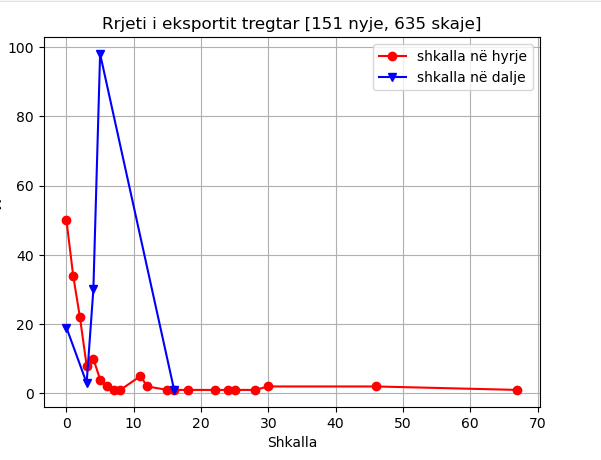
\includegraphics{./Figs/trade5.png}
\end{frame}

\begin{frame}{Vizualizimi i Nyjeve dhe Skajeve}
\protect\hypertarget{vizualizimi-i-nyjeve-dhe-skajeve}{}
\begin{itemize}
\item
  Gjenerimi i vizualizimeve të mira të rrjeteve nuk është i lehtë.
\item
  Kur një rrjet rritet në numër të nyjeve dhe shkallë, mbivendosja bëhet
  e pashmangshme.
\end{itemize}
\end{frame}

\begin{frame}{Vizualizimi i Nyjeve dhe Skajeve}
\protect\hypertarget{vizualizimi-i-nyjeve-dhe-skajeve-1}{}
\begin{itemize}
\item
  Libraria ofron funksionalitet për vizualizim të avancuar
\item
  Me grafet hapësinore, është e nevojshme të zgjidhni një paraqitje për
  të rregulluar nyjet në një mënyrë të përshtatshme.
\end{itemize}
\end{frame}

\begin{frame}[fragile]{Vizualizimi i Nyjeve dhe Skajeve}
\protect\hypertarget{vizualizimi-i-nyjeve-dhe-skajeve-2}{}
python\AddToHookNext{env/Highlighting/begin}{\tiny}

\begin{Shaded}
\begin{Highlighting}[]
\CommentTok{\# përkufizoni funksionin e ripërdorshëm për të vizatuar paraqitjen e rrjetit}
\KeywordTok{def}\NormalTok{ plot\_graph(g, title, edge\_label\_attribute, layout}\OperatorTok{=}\StringTok{\textquotesingle{}spring\textquotesingle{}}\NormalTok{, fig\_sz}\OperatorTok{=}\DecValTok{10}\NormalTok{):}
    \CommentTok{"""}
\CommentTok{    Funksioni për të vizatuar një grafik të drejtuar me vlera të përshtatshme të parazgjedhura.}
\CommentTok{    @ g: një grafik}
\CommentTok{    @ title: titulli i grafikut}
\CommentTok{    @ edge\_label\_attribute: emri i atributit të skajit që do të përdoret si etiketa e skajit}
\CommentTok{    @ layout: paraqitja e rrjetit që do të përdoret}
\CommentTok{    @ fig\_sz: madhësia e kanavacës}
\CommentTok{    """}
    \CommentTok{\# gjeneroni pozicionet e nyjeve bazuar në paraqitjen e zgjedhur}
    \ControlFlowTok{if}\NormalTok{ layout }\OperatorTok{==} \StringTok{\textquotesingle{}spring\textquotesingle{}}\NormalTok{:}
\NormalTok{        pos }\OperatorTok{=}\NormalTok{ nx.spring\_layout(g, k}\OperatorTok{=}\FloatTok{0.55}\NormalTok{, iterations}\OperatorTok{=}\DecValTok{30}\NormalTok{)}
    \ControlFlowTok{elif}\NormalTok{ layout }\OperatorTok{==} \StringTok{\textquotesingle{}circular\textquotesingle{}}\NormalTok{:}
\NormalTok{        pos }\OperatorTok{=}\NormalTok{ nx.circular\_layout(g)}
    \ControlFlowTok{else}\NormalTok{:}
        \ControlFlowTok{raise} \PreprocessorTok{ValueError}\NormalTok{(}\StringTok{"Paraqitje e pavlefshme"}\NormalTok{)}
\end{Highlighting}
\end{Shaded}
\end{frame}

\begin{frame}[fragile]{Vizualizimi i Nyjeve dhe Skajeve (vazhdim)}
\protect\hypertarget{vizualizimi-i-nyjeve-dhe-skajeve-vazhdim}{}
python\AddToHookNext{env/Highlighting/begin}{\tiny}

\begin{Shaded}
\begin{Highlighting}[]
    \CommentTok{\# rregulloni figurën}
\NormalTok{    plt.figure(figsize}\OperatorTok{=}\NormalTok{(fig\_sz, fig\_sz))}
    \CommentTok{\# hapni vizatimin}
\NormalTok{    nx.draw\_networkx(g, pos}\OperatorTok{=}\NormalTok{pos, node\_color}\OperatorTok{=}\StringTok{\textquotesingle{}lightblue\textquotesingle{}}\NormalTok{, alpha}\OperatorTok{=}\FloatTok{.8}\NormalTok{)}
    \CommentTok{\# nxirrni etiketat e skajeve}
\NormalTok{    edge\_labels }\OperatorTok{=}\NormalTok{ nx.get\_edge\_attributes(g, edge\_label\_attribute)}
    \CommentTok{\# vizatoni etiketat e skajeve}
\NormalTok{    nx.draw\_networkx\_edge\_labels(g, pos}\OperatorTok{=}\NormalTok{pos, edge\_labels}\OperatorTok{=}\NormalTok{edge\_labels, alpha}\OperatorTok{=}\FloatTok{.6}\NormalTok{)}
    \CommentTok{\# vizatoni skajet}
\NormalTok{    nx.draw\_networkx\_edges(g, pos}\OperatorTok{=}\NormalTok{pos, arrows}\OperatorTok{=}\VariableTok{True}\NormalTok{, alpha}\OperatorTok{=}\FloatTok{.6}\NormalTok{, edge\_color}\OperatorTok{=}\StringTok{\textquotesingle{}lightgray\textquotesingle{}}\NormalTok{)}
\NormalTok{    plt.title(title)}
\NormalTok{    plt.show()}
\end{Highlighting}
\end{Shaded}
\end{frame}

\begin{frame}[fragile]{Vizualizimi i Nyjeve dhe Skajeve (vazhdim)}
\protect\hypertarget{vizualizimi-i-nyjeve-dhe-skajeve-vazhdim-1}{}
python\AddToHookNext{env/Highlighting/begin}{\tiny}

\begin{Shaded}
\begin{Highlighting}[]
\CommentTok{\# vizatoni grafikun me dy paraqitje të ndryshme}
\NormalTok{plot\_graph(trade\_export\_g, }\StringTok{"Rrjeti i eksportit (}\SpecialCharTok{\% i}\StringTok{ eksportit total)"}\NormalTok{, }\StringTok{\textquotesingle{}2018\textquotesingle{}}\NormalTok{, }\StringTok{\textquotesingle{}circular\textquotesingle{}}\NormalTok{, fig\_sz}\OperatorTok{=}\DecValTok{40}\NormalTok{)}
\NormalTok{plot\_graph(trade\_import\_g, }\StringTok{"Rrjeti i importit (}\SpecialCharTok{\% i}\StringTok{ importit total)"}\NormalTok{, }\StringTok{\textquotesingle{}2018\textquotesingle{}}\NormalTok{, }\StringTok{\textquotesingle{}spring\textquotesingle{}}\NormalTok{, fig\_sz}\OperatorTok{=}\DecValTok{40}\NormalTok{)}
\end{Highlighting}
\end{Shaded}
\end{frame}

\begin{frame}{Vizualizimi i Nyjeve dhe Skajeve (vazhdim)}
\protect\hypertarget{vizualizimi-i-nyjeve-dhe-skajeve-vazhdim-2}{}
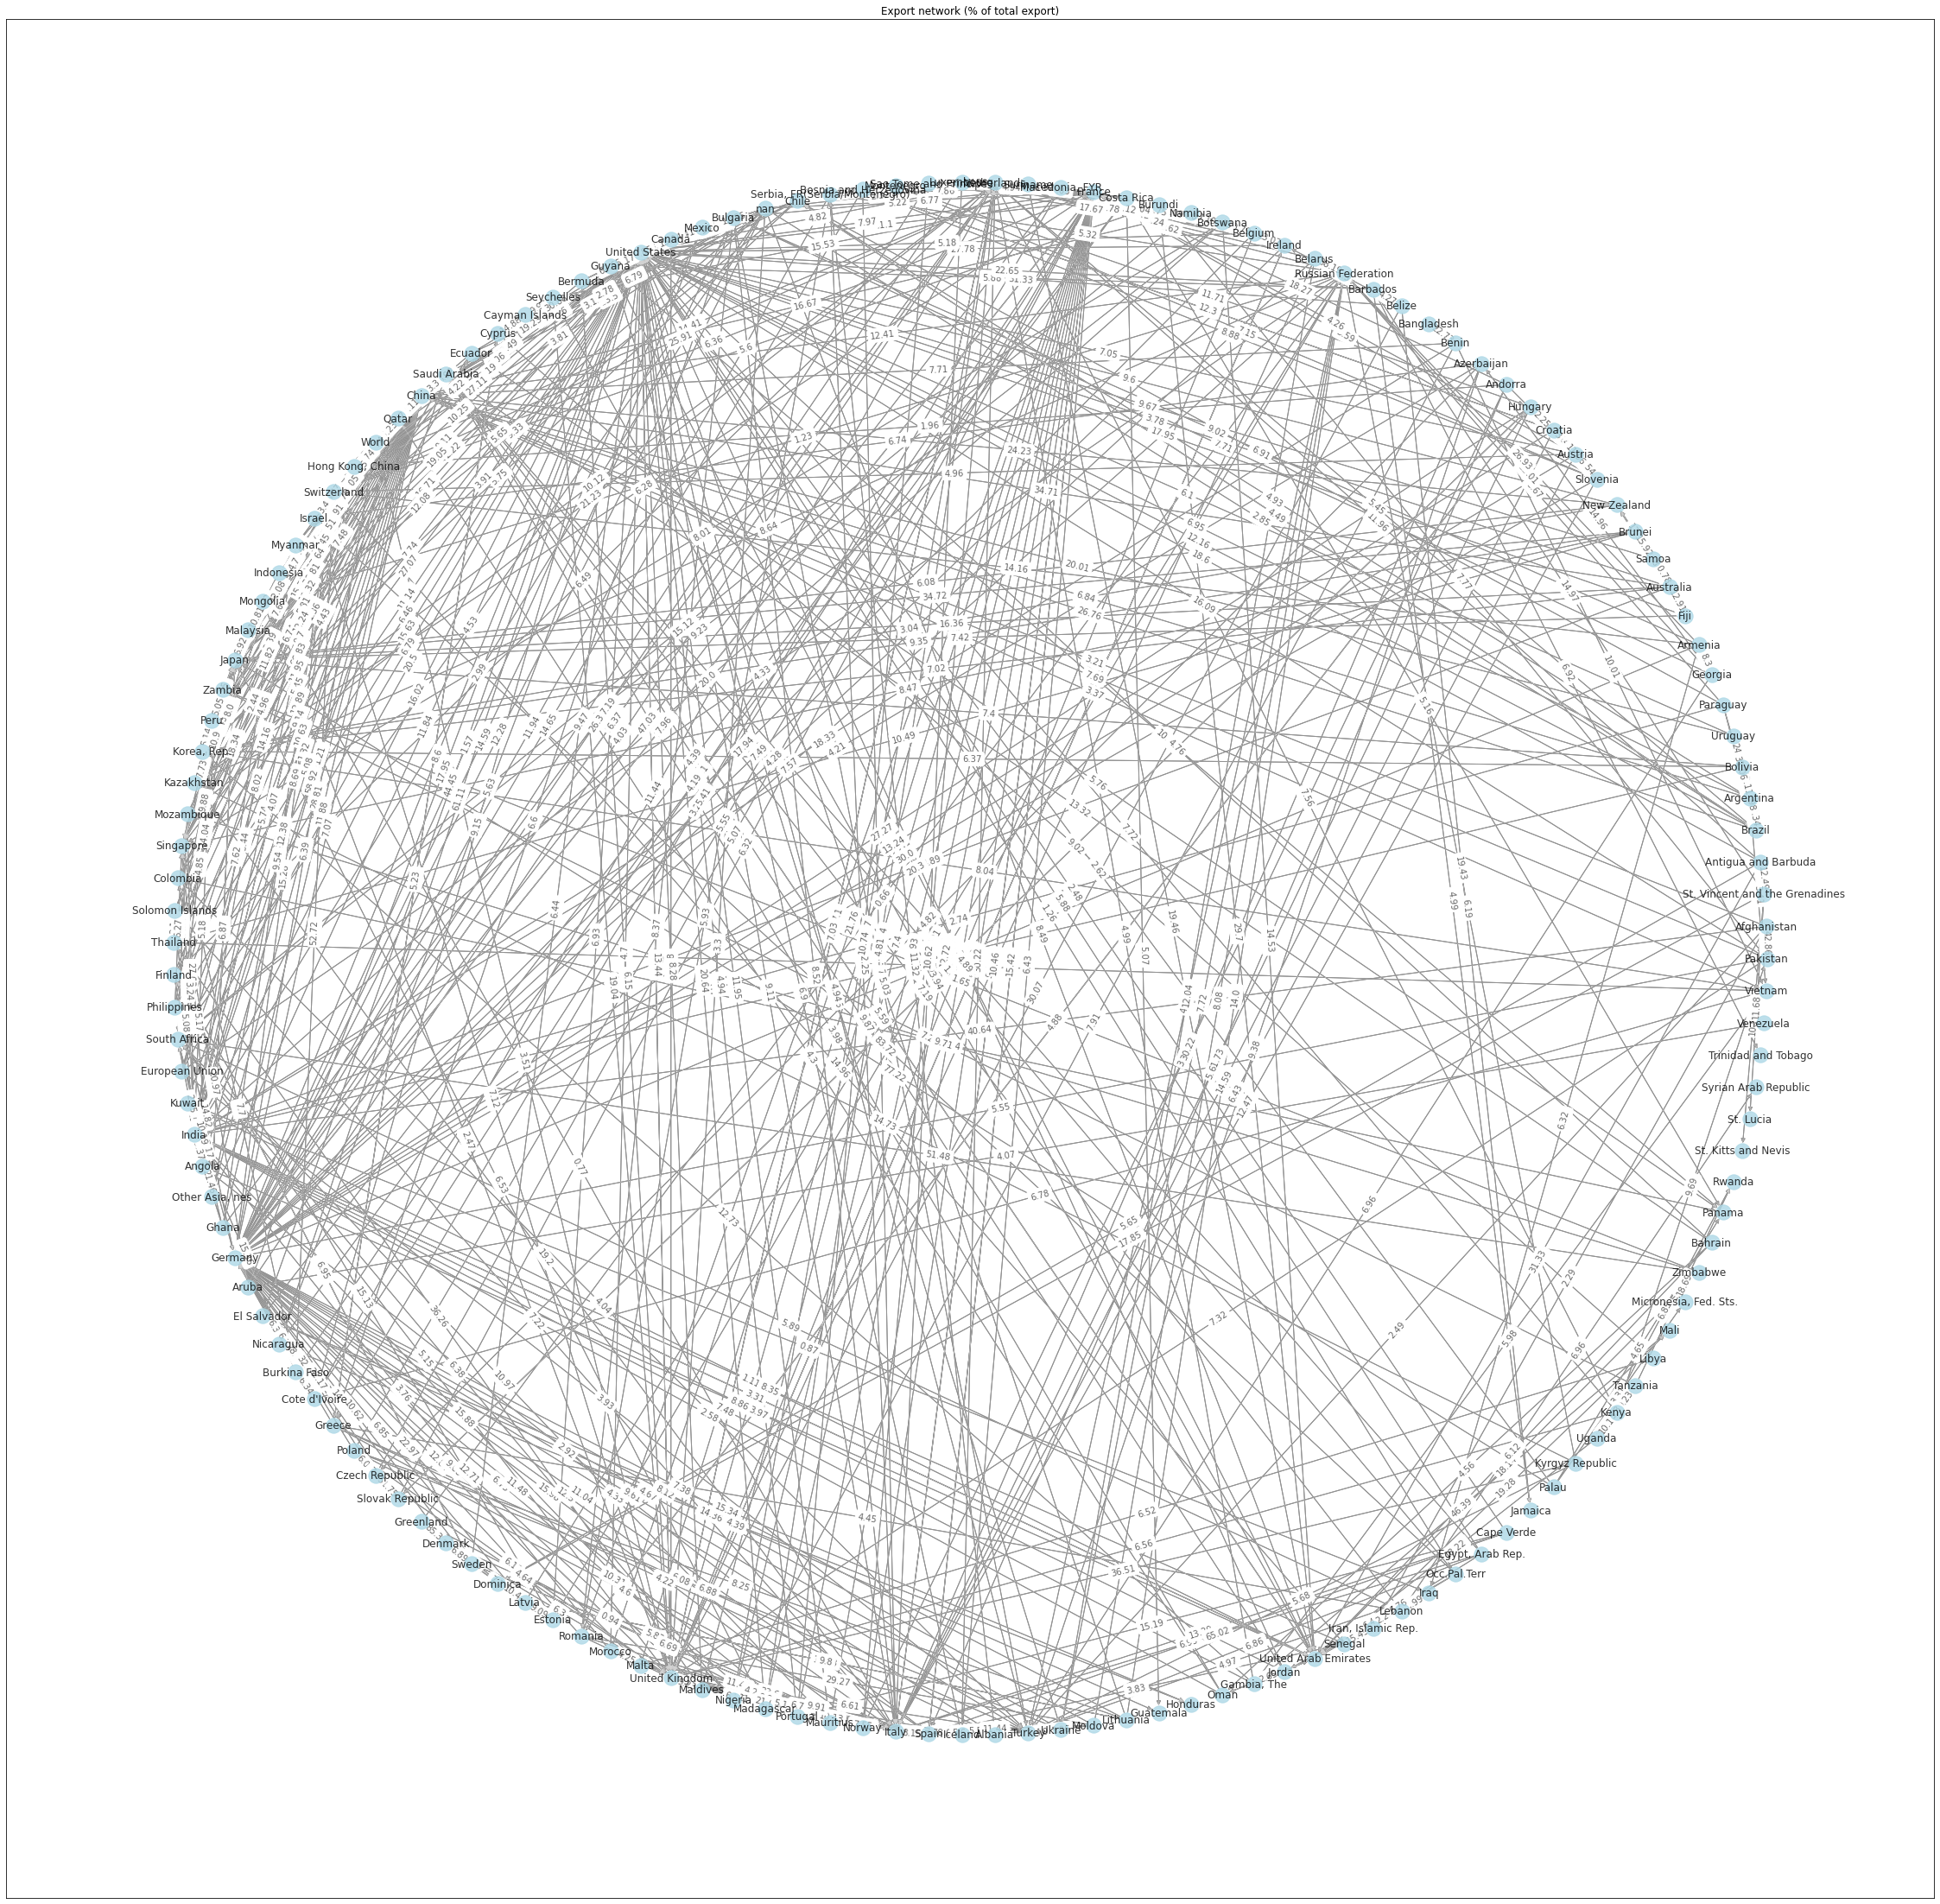
\includegraphics{./Figs/difrrjet.png}
\end{frame}

\begin{frame}{Vizualizimi i Nyjeve dhe Skajeve}
\protect\hypertarget{vizualizimi-i-nyjeve-dhe-skajeve-3}{}
\begin{itemize}
\item
  Këto vizualizime në thelb janë të padobishme pasi nuk mund të dallojmë
  strukturën e rrjeteve.
\item
  Një strategji për të vizualizuar një rrjet të madh është të përfshini
  vetëm nyje të lidhura relativisht.
\item
  Për shembull, le të zgjedhim nyje me shkallë të lartë nga grafiku
  \textbf{trade\_export\_g}:
\end{itemize}
\end{frame}

\begin{frame}[fragile]{Vizualizimi i Nyjeve dhe Skajeve}
\protect\hypertarget{vizualizimi-i-nyjeve-dhe-skajeve-4}{}
python\AddToHookNext{env/Highlighting/begin}{\tiny}

\begin{Shaded}
\begin{Highlighting}[]
\CommentTok{\# zgjedhni nyjet me shkallë të lartë}
\NormalTok{degrees }\OperatorTok{=}\NormalTok{ trade\_export\_g.degree()}
\NormalTok{nodes\_to\_remove }\OperatorTok{=}\NormalTok{ [n }\ControlFlowTok{for}\NormalTok{ n, degree }\KeywordTok{in}\NormalTok{ degrees }\ControlFlowTok{if}\NormalTok{ degrees[n] }\OperatorTok{\textless{}} \DecValTok{20}\NormalTok{]}

\CommentTok{\# kopjoni dhe hiqni nyjet nga grafiku}
\NormalTok{hideg\_trade\_export\_g }\OperatorTok{=}\NormalTok{ trade\_export\_g.copy()}
\NormalTok{hideg\_trade\_export\_g.remove\_nodes\_from(nodes\_to\_remove)}

\CommentTok{\# shtypni informacionin e grafikut të shkallës së lartë}
\KeywordTok{def}\NormalTok{ print\_graph\_info(g):}
\NormalTok{    num\_nodes }\OperatorTok{=}\NormalTok{ g.number\_of\_nodes()}
\NormalTok{    num\_edges }\OperatorTok{=}\NormalTok{ g.number\_of\_edges()}
\NormalTok{    avg\_in\_degree }\OperatorTok{=} \BuiltInTok{sum}\NormalTok{(}\BuiltInTok{dict}\NormalTok{(g.in\_degree()).values()) }\OperatorTok{/}\NormalTok{ num\_nodes}
\NormalTok{    avg\_out\_degree }\OperatorTok{=} \BuiltInTok{sum}\NormalTok{(}\BuiltInTok{dict}\NormalTok{(g.out\_degree()).values()) }\OperatorTok{/}\NormalTok{ num\_nodes}

    \BuiltInTok{print}\NormalTok{(}\SpecialStringTok{f"Name:"}\NormalTok{)}
    \BuiltInTok{print}\NormalTok{(}\SpecialStringTok{f"Type: }\SpecialCharTok{\{}\BuiltInTok{type}\NormalTok{(g)}\SpecialCharTok{.}\VariableTok{\_\_name\_\_}\SpecialCharTok{\}}\SpecialStringTok{"}\NormalTok{)}
    \BuiltInTok{print}\NormalTok{(}\SpecialStringTok{f"Number of nodes: }\SpecialCharTok{\{}\NormalTok{num\_nodes}\SpecialCharTok{\}}\SpecialStringTok{"}\NormalTok{)}
    \BuiltInTok{print}\NormalTok{(}\SpecialStringTok{f"Number of edges: }\SpecialCharTok{\{}\NormalTok{num\_edges}\SpecialCharTok{\}}\SpecialStringTok{"}\NormalTok{)}
    \BuiltInTok{print}\NormalTok{(}\SpecialStringTok{f"Average in degree: }\SpecialCharTok{\{}\NormalTok{avg\_in\_degree}\SpecialCharTok{:.4f\}}\SpecialStringTok{"}\NormalTok{)}
    \BuiltInTok{print}\NormalTok{(}\SpecialStringTok{f"Average out degree: }\SpecialCharTok{\{}\NormalTok{avg\_out\_degree}\SpecialCharTok{:.4f\}}\SpecialStringTok{"}\NormalTok{)}

\NormalTok{print\_graph\_info(hideg\_trade\_export\_g)}
\end{Highlighting}
\end{Shaded}
\end{frame}

\begin{frame}{Vizualizimi i Nyjeve dhe Skajeve}
\protect\hypertarget{vizualizimi-i-nyjeve-dhe-skajeve-5}{}
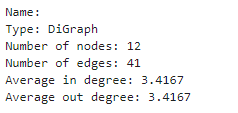
\includegraphics{./Figs/difrrjet1.png}
\end{frame}

\begin{frame}{Vizualizimi i Nyjeve dhe Skajeve}
\protect\hypertarget{vizualizimi-i-nyjeve-dhe-skajeve-6}{}
Grafiku me shkallë të lartë është më i lehtë për t'u vizatuar dhe ne
mund të shohim lidhjet midis vendeve me shkallë të lartë:
\end{frame}

\begin{frame}[fragile]{Vizualizimi i Nyjeve dhe Skajeve}
\protect\hypertarget{vizualizimi-i-nyjeve-dhe-skajeve-7}{}
python\AddToHookNext{env/Highlighting/begin}{\tiny}

\begin{Shaded}
\begin{Highlighting}[]
\CommentTok{\# grafiku i shkallës së lartë}
\NormalTok{plot\_graph(hideg\_trade\_export\_g, }\StringTok{"Rrjeti i eksportit (}\SpecialCharTok{\% i}\StringTok{ eksportit total)"}\NormalTok{, }\StringTok{\textquotesingle{}2018\textquotesingle{}}\NormalTok{, }\StringTok{\textquotesingle{}spring\textquotesingle{}}\NormalTok{, fig\_sz}\OperatorTok{=}\DecValTok{10}\NormalTok{)}
\end{Highlighting}
\end{Shaded}
\end{frame}

\begin{frame}{Vizualizimi i Nyjeve dhe Skajeve}
\protect\hypertarget{vizualizimi-i-nyjeve-dhe-skajeve-8}{}
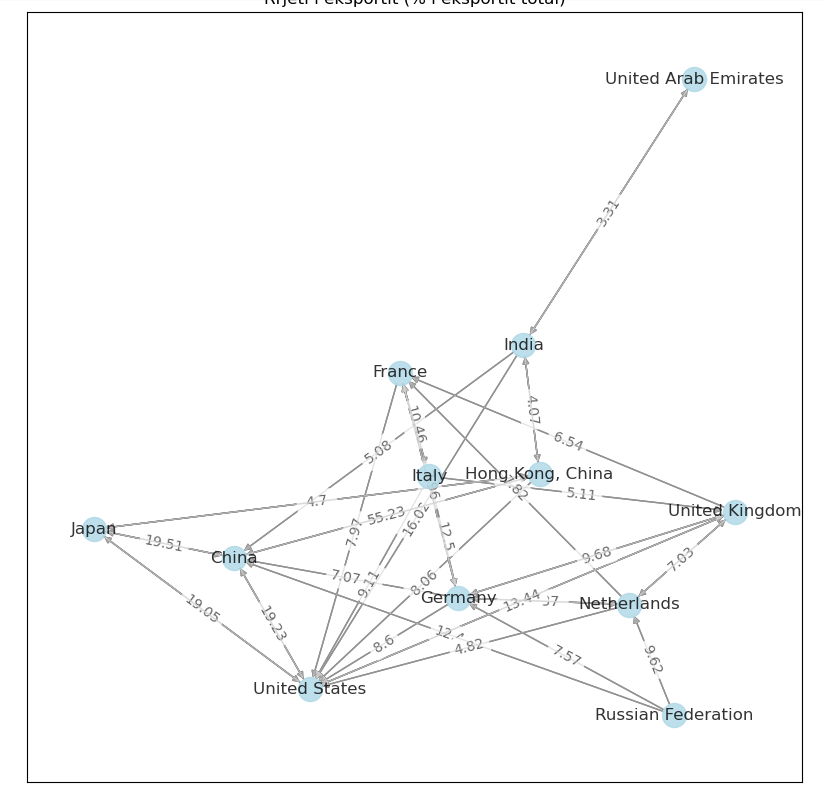
\includegraphics{./Figs/difrrjet2.png}
\end{frame}

\begin{frame}[fragile]{Vizualizimi i Nyjeve dhe Skajeve}
\protect\hypertarget{vizualizimi-i-nyjeve-dhe-skajeve-9}{}
Një qasje tjetër është të zgjidhni nën-grafikë, për shembull fqinjët e
një nyje të synuar:

python\AddToHookNext{env/Highlighting/begin}{\tiny}

\begin{Shaded}
\begin{Highlighting}[]
\CommentTok{\# tregoni nën{-}grafikë për secilin vend me shkallë të lartë}
\ControlFlowTok{for}\NormalTok{ country }\KeywordTok{in}\NormalTok{ hideg\_trade\_export\_g.nodes:}
    \CommentTok{\# nxirrni nën{-}grafikun për rrjetin e eksportit të një vendi}
    \CommentTok{\# skajet në dalje}
\NormalTok{    edges }\OperatorTok{=}\NormalTok{ trade\_export\_g.out\_edges(country, data}\OperatorTok{=}\VariableTok{True}\NormalTok{)}
\NormalTok{    g }\OperatorTok{=}\NormalTok{ nx.DiGraph(edges)}
\NormalTok{    plot\_graph(g, }\StringTok{"Rrjeti i eksportit nga}\CharTok{\textbackslash{}n}\StringTok{"} \OperatorTok{+}\NormalTok{ country }\OperatorTok{+} \StringTok{\textquotesingle{} (}\SpecialCharTok{\% i}\StringTok{ eksportit total)\textquotesingle{}}\NormalTok{, }\StringTok{\textquotesingle{}2018\textquotesingle{}}\NormalTok{, fig\_sz}\OperatorTok{=}\DecValTok{6}\NormalTok{)}
    \CommentTok{\# skajet në hyrje}
\NormalTok{    edges }\OperatorTok{=}\NormalTok{ trade\_export\_g.in\_edges(country, data}\OperatorTok{=}\VariableTok{True}\NormalTok{)}
\NormalTok{    g }\OperatorTok{=}\NormalTok{ nx.DiGraph(edges)}
\NormalTok{    plot\_graph(g, }\StringTok{"Rrjeti i eksportit për}\CharTok{\textbackslash{}n}\StringTok{"} \OperatorTok{+}\NormalTok{ country }\OperatorTok{+} \StringTok{\textquotesingle{} (}\SpecialCharTok{\% i}\StringTok{ eksportit total)\textquotesingle{}}\NormalTok{, }\StringTok{\textquotesingle{}2018\textquotesingle{}}\NormalTok{, fig\_sz}\OperatorTok{=}\DecValTok{6}\NormalTok{)}
\end{Highlighting}
\end{Shaded}
\end{frame}

\begin{frame}{Vizualizimi i Nyjeve dhe Skajeve}
\protect\hypertarget{vizualizimi-i-nyjeve-dhe-skajeve-10}{}
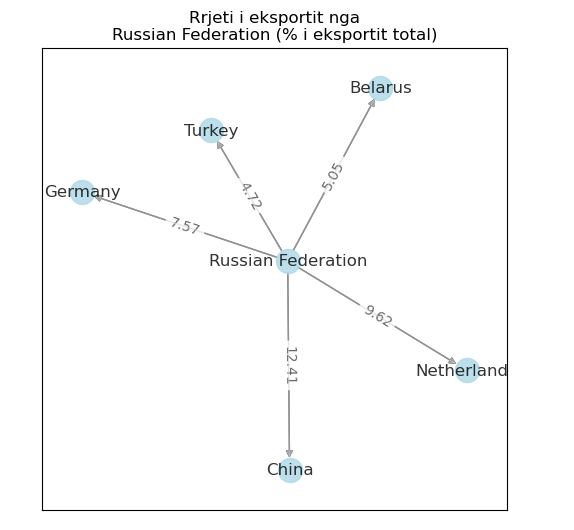
\includegraphics{./Figs/difrrjet3.png}
\end{frame}

\begin{frame}{Eksportimi i grafikut}
\protect\hypertarget{eksportimi-i-grafikut}{}
\begin{itemize}
\item
  Shpesh është e nevojshme të eksportoni një grafik në një format
  standard të skedarit
\item
  \textbf{networkX} supporton shumë formate.
\item
  Ndër formatet më të supportuara janë \textbf{GraphML} dhe
  \textbf{GEXF}, të dy bazuar në XML.
\end{itemize}
\end{frame}

\begin{frame}{Eksportimi i grafikut}
\protect\hypertarget{eksportimi-i-grafikut-1}{}
Ekzaminoni skedarët e eksportuar me një redaktues teksti për të parë se
si kodohen të dhënat.
\end{frame}

\begin{frame}[fragile]{Eksportimi i grafikut}
\protect\hypertarget{eksportimi-i-grafikut-2}{}
python\AddToHookNext{env/Highlighting/begin}{\tiny}

\begin{Shaded}
\begin{Highlighting}[]
\CommentTok{\# eksportoni grafikun si GraphML dhe GEXF}
\NormalTok{nx.write\_graphml(hideg\_trade\_export\_g, }\StringTok{"tmp/street\_network.graphml"}\NormalTok{)}
\NormalTok{nx.write\_gexf(hideg\_trade\_export\_g, }\StringTok{"tmp/street\_network.gexf"}\NormalTok{)}
\end{Highlighting}
\end{Shaded}
\end{frame}

\begin{frame}{Qëndra e Nyjeve}
\protect\hypertarget{quxebndra-e-nyjeve}{}
\begin{itemize}
\tightlist
\item
  Ne mund të përdorim \textbf{networkX} për të llogaritur metrikat e
  rrjetit, për shembull për të parë qendrën e ndërmjetësimit të vendeve
  në të dy rrjetet e ndryshme që përfaqësojnë importin dhe eksportin:
\end{itemize}
\end{frame}

\begin{frame}[fragile]{Qëndra e Nyjeve}
\protect\hypertarget{quxebndra-e-nyjeve-1}{}
python\AddToHookNext{env/Highlighting/begin}{\tiny}

\begin{Shaded}
\begin{Highlighting}[]
\CommentTok{\# llogarisni qendrën e ndërmjetësimit bazuar në dendësinë e nyjeve}
\NormalTok{country\_centrality }\OperatorTok{=}\NormalTok{ nx.algorithms.centrality.betweenness\_centrality(trade\_export\_g)}

\CommentTok{\# konvertoni të dhënat në një kuadër të dhënash}
\NormalTok{country\_centrality\_df }\OperatorTok{=}\NormalTok{ pd.DataFrame.from\_dict(country\_centrality, }
\NormalTok{                                orient}\OperatorTok{=}\StringTok{\textquotesingle{}index\textquotesingle{}}\NormalTok{, columns}\OperatorTok{=}\NormalTok{[}\StringTok{\textquotesingle{}betw\_centrality\_export\textquotesingle{}}\NormalTok{])}
\NormalTok{country\_centrality\_df[}\StringTok{\textquotesingle{}country\textquotesingle{}}\NormalTok{] }\OperatorTok{=}\NormalTok{ country\_centrality\_df.index}

\CommentTok{\# renditni dhe tregoni rezultatet}
\NormalTok{country\_centrality\_df }\OperatorTok{=}\NormalTok{ country\_centrality\_df.sort\_values(}\StringTok{\textquotesingle{}betw\_centrality\_export\textquotesingle{}}\NormalTok{, ascending}\OperatorTok{=}\VariableTok{False}\NormalTok{)}
\NormalTok{country\_centrality\_df.head(}\DecValTok{10}\NormalTok{)}
\end{Highlighting}
\end{Shaded}
\end{frame}

\begin{frame}[fragile]{Qëndra e Nyjeve}
\protect\hypertarget{quxebndra-e-nyjeve-2}{}
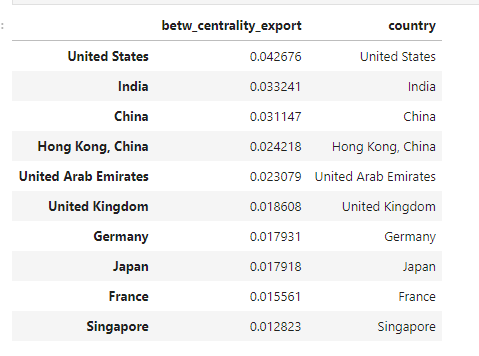
\includegraphics{./Figs/qnyje.png} \#\# Importo Rrjetin

python\AddToHookNext{env/Highlighting/begin}{\tiny}

\begin{Shaded}
\begin{Highlighting}[]
\CommentTok{\# llogarisni qendrën e ndërmjetësimit të rrjetit të importit}
\NormalTok{country\_centrality }\OperatorTok{=}\NormalTok{ nx.algorithms.centrality.betweenness\_centrality(trade\_import\_g)}
\NormalTok{imp\_df }\OperatorTok{=}\NormalTok{ pd.DataFrame.from\_dict(country\_centrality, }
\NormalTok{                            orient}\OperatorTok{=}\StringTok{\textquotesingle{}index\textquotesingle{}}\NormalTok{, columns}\OperatorTok{=}\NormalTok{[}\StringTok{\textquotesingle{}betw\_centrality\_import\textquotesingle{}}\NormalTok{])}

\CommentTok{\# renditni dhe tregoni rezultatet}
\NormalTok{imp\_df }\OperatorTok{=}\NormalTok{ imp\_df.sort\_values(}\StringTok{\textquotesingle{}betw\_centrality\_import\textquotesingle{}}\NormalTok{, ascending}\OperatorTok{=}\VariableTok{False}\NormalTok{)}
\NormalTok{imp\_df[}\StringTok{\textquotesingle{}country\textquotesingle{}}\NormalTok{] }\OperatorTok{=}\NormalTok{ imp\_df.index}
\NormalTok{imp\_df.head(}\DecValTok{10}\NormalTok{)}
\end{Highlighting}
\end{Shaded}
\end{frame}

\begin{frame}{Importo Rrjetin}
\protect\hypertarget{importo-rrjetin}{}
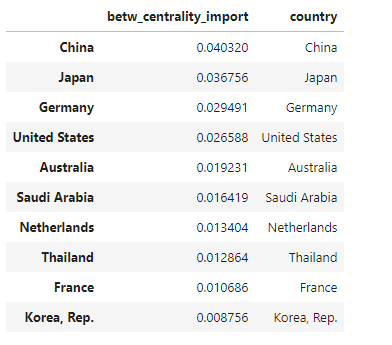
\includegraphics{./Figs/qnyje1.png}
\end{frame}

\begin{frame}[fragile]{Kombinimi i Treguesve për të Krahasuar}
\protect\hypertarget{kombinimi-i-treguesve-puxebr-tuxeb-krahasuar}{}
python\AddToHookNext{env/Highlighting/begin}{\tiny}

\begin{Shaded}
\begin{Highlighting}[]
\CommentTok{\# kombinoni dy treguesit për t\textquotesingle{}i krahasuar ata}
\NormalTok{impexp\_df }\OperatorTok{=}\NormalTok{ country\_centrality\_df.merge(imp\_df, on}\OperatorTok{=}\StringTok{\textquotesingle{}country\textquotesingle{}}\NormalTok{)}
\NormalTok{impexp\_df }\OperatorTok{=}\NormalTok{ impexp\_df[[}\StringTok{\textquotesingle{}country\textquotesingle{}}\NormalTok{,}\StringTok{\textquotesingle{}betw\_centrality\_import\textquotesingle{}}\NormalTok{,}\StringTok{\textquotesingle{}betw\_centrality\_export\textquotesingle{}}\NormalTok{]]}
\NormalTok{impexp\_df }\OperatorTok{=}\NormalTok{ impexp\_df.sort\_values(}\StringTok{\textquotesingle{}betw\_centrality\_export\textquotesingle{}}\NormalTok{, ascending}\OperatorTok{=}\VariableTok{False}\NormalTok{)}
\NormalTok{impexp\_df.to\_csv(}\StringTok{\textquotesingle{}tmp/trade\_importexport\_centrality\_2018.csv\textquotesingle{}}\NormalTok{)}
\NormalTok{impexp\_df.head(}\DecValTok{10}\NormalTok{)}
\end{Highlighting}
\end{Shaded}
\end{frame}

\begin{frame}{Kombinimi i Treguesve për të Krahasuar}
\protect\hypertarget{kombinimi-i-treguesve-puxebr-tuxeb-krahasuar-1}{}
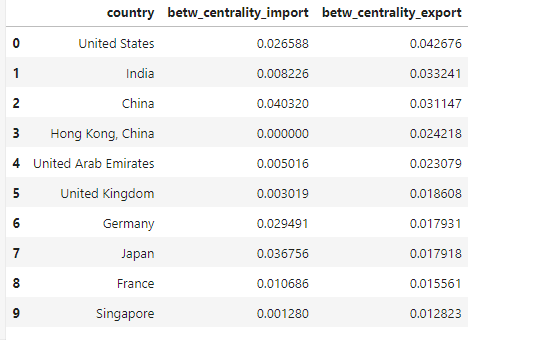
\includegraphics{./Figs/qnyje2.png}
\end{frame}

\begin{frame}{Rrjetet Rrugore}
\protect\hypertarget{rrjetet-rrugore}{}
\begin{itemize}
\item
  Rrjetet rrugore janë një lloj rrjeti që është veçanërisht i
  rëndësishëm në analizën e të dhënave gjeografike.
\item
  Libraria \textbf{osmnx} ofron funksione për të nxjerrë lehtësisht
  rrjetet rrugore nga \textbf{OpenStreetMap}.
\end{itemize}
\end{frame}

\begin{frame}{Rrjetet Rrugore}
\protect\hypertarget{rrjetet-rrugore-1}{}
\begin{itemize}
\item
  Mënyra më efikase për të ruajtur këto rrjete kur punoni në Python
  është formati \textbf{pickle}.
\item
  Do të përdorim skedarë pickle të kompresuar.
\item
  Shumë formate të tjera rrjeti ekzistojnë, duke përfshirë GeoPackages
  dhe GraphML, që mund të përdoren .
\end{itemize}
\end{frame}

\begin{frame}[fragile]{Merrni Rrjetet Rrugore}
\protect\hypertarget{merrni-rrjetet-rrugore}{}
python\AddToHookNext{env/Highlighting/begin}{\tiny}

\begin{Shaded}
\begin{Highlighting}[]
\ImportTok{import}\NormalTok{ osmnx }\ImportTok{as}\NormalTok{ ox}
\ImportTok{import}\NormalTok{ pickle}

\CommentTok{\# Emri i vendit të synuar}
\NormalTok{place\_name }\OperatorTok{=} \StringTok{"City of London, UK"}

\CommentTok{\# Shkarkoni rrjetin rrugor nga OpenStreetMap bazuar në një emër vendi}
\NormalTok{graph }\OperatorTok{=}\NormalTok{ ox.graph\_from\_place(place\_name, network\_type}\OperatorTok{=}\StringTok{\textquotesingle{}drive\textquotesingle{}}\NormalTok{)}

\CommentTok{\# Ruani rrjetin në disk duke përdorur gzip (.gz) për të zvogëluar madhësinë e skedarit}
\NormalTok{net\_file }\OperatorTok{=} \StringTok{"data/streets\_citylondon.gpik"}

\CommentTok{\# Use pickle to write the graph to a file}
\ControlFlowTok{with} \BuiltInTok{open}\NormalTok{(net\_file, }\StringTok{\textquotesingle{}wb\textquotesingle{}}\NormalTok{) }\ImportTok{as}\NormalTok{ f:}
\NormalTok{    pickle.dump(graph, f)}

\BuiltInTok{print}\NormalTok{(}\StringTok{"Skedari i grafikut të rrugëve në"}\NormalTok{, place\_name, }\StringTok{"shkarkuar në"}\NormalTok{, net\_file)}
\end{Highlighting}
\end{Shaded}
\end{frame}

\begin{frame}[fragile]{Merrni Rrjetet Rrugore}
\protect\hypertarget{merrni-rrjetet-rrugore-1}{}
python\AddToHookNext{env/Highlighting/begin}{\tiny}

\begin{Shaded}
\begin{Highlighting}[]
\CommentTok{\# \textquotesingle{}del\textquotesingle{} (fshij) shkatërron një objekt. Është e dobishme për të siguruar që ky objekt}
\CommentTok{\# nuk mund të përdoret në qeliza të tjera gabimisht.}
\KeywordTok{del}\NormalTok{ graph, net\_file}
\end{Highlighting}
\end{Shaded}
\end{frame}

\begin{frame}[fragile]{Merrni Rrjetet Rrugore}
\protect\hypertarget{merrni-rrjetet-rrugore-2}{}
Në mënyrë alternative, paketa supporton një \textbf{point and radius
search} bazuar në adresa ose nga poligonet:

python\AddToHookNext{env/Highlighting/begin}{\tiny}

\begin{Shaded}
\begin{Highlighting}[]
\ImportTok{import}\NormalTok{ osmnx }\ImportTok{as}\NormalTok{ ox}
\ImportTok{import}\NormalTok{ pickle}
\ImportTok{import}\NormalTok{ gzip}

\CommentTok{\# Vendndodhja e Birkbeck, rreze 1 km}
\NormalTok{radius\_m }\OperatorTok{=} \DecValTok{1000}
\NormalTok{graph }\OperatorTok{=}\NormalTok{ ox.graph\_from\_address(}\StringTok{\textquotesingle{}Malet St, London, UK\textquotesingle{}}\NormalTok{, network\_type}\OperatorTok{=}\StringTok{\textquotesingle{}drive\textquotesingle{}}\NormalTok{, dist}\OperatorTok{=}\NormalTok{radius\_m)}

\CommentTok{\# Ruani rrjetin në disk duke përdorur gzip (.gz) për të zvogëluar madhësinë e skedarit}
\NormalTok{net\_file }\OperatorTok{=} \StringTok{"data/streets\_birkbeck\_1km.gpik.gz"}

\CommentTok{\# Use pickle to write the graph to a compressed file}
\ControlFlowTok{with}\NormalTok{ gzip.}\BuiltInTok{open}\NormalTok{(net\_file, }\StringTok{\textquotesingle{}wb\textquotesingle{}}\NormalTok{) }\ImportTok{as}\NormalTok{ f:}
\NormalTok{    pickle.dump(graph, f)}

\BuiltInTok{print}\NormalTok{(}\SpecialStringTok{f"Rrjeti rrugor i ruajtur në }\SpecialCharTok{\{}\NormalTok{net\_file}\SpecialCharTok{\}}\SpecialStringTok{"}\NormalTok{)}

\CommentTok{\# Delete the graph object to free up memory}
\KeywordTok{del}\NormalTok{ graph}
\end{Highlighting}
\end{Shaded}
\end{frame}

\begin{frame}{Vizato Rrjetin e Rrugës}
\protect\hypertarget{vizato-rrjetin-e-rruguxebs}{}
\begin{itemize}
\item
  Rrjeti rrugor shprehet si
  \textbf{networkx.classes.multidigraph.MultiDiGraph}.
\item
  Le të ngarkojmë një skedar \textbf{pickle} dhe të vizatojmë rrjetin.
\end{itemize}
\end{frame}

\begin{frame}[fragile]{Vizato Rrjetin e Rrugës}
\protect\hypertarget{vizato-rrjetin-e-rruguxebs-1}{}
python\AddToHookNext{env/Highlighting/begin}{\tiny}

\begin{Shaded}
\begin{Highlighting}[]
\ImportTok{import}\NormalTok{ pickle}
\ImportTok{import}\NormalTok{ gzip}

\CommentTok{\# Load the graph from the compressed file}
\NormalTok{net\_file }\OperatorTok{=} \StringTok{"data/streets\_birkbeck\_1km.gpik.gz"}
\ControlFlowTok{with}\NormalTok{ gzip.}\BuiltInTok{open}\NormalTok{(net\_file, }\StringTok{\textquotesingle{}rb\textquotesingle{}}\NormalTok{) }\ImportTok{as}\NormalTok{ f:}
\NormalTok{    streets\_g }\OperatorTok{=}\NormalTok{ pickle.load(f)}

\CommentTok{\# Print the number of nodes and edges in the graph}
\BuiltInTok{print}\NormalTok{(}\StringTok{"N i nyjeve:"}\NormalTok{, }\BuiltInTok{len}\NormalTok{(streets\_g.nodes))}
\BuiltInTok{print}\NormalTok{(}\StringTok{"N i skajeve:"}\NormalTok{, }\BuiltInTok{len}\NormalTok{(streets\_g.edges))}
\end{Highlighting}
\end{Shaded}
\end{frame}

\begin{frame}[fragile]{Vizato Rrjetin e Rrugës}
\protect\hypertarget{vizato-rrjetin-e-rruguxebs-2}{}
python\AddToHookNext{env/Highlighting/begin}{\tiny}

\begin{Shaded}
\begin{Highlighting}[]
\CommentTok{\# vizatoni rrjetin}
\NormalTok{osmnx.plot\_graph(streets\_g, figsize}\OperatorTok{=}\NormalTok{(}\DecValTok{10}\NormalTok{,}\DecValTok{10}\NormalTok{))}
\end{Highlighting}
\end{Shaded}
\end{frame}

\begin{frame}{Vizato Rrjetin e Rrugës}
\protect\hypertarget{vizato-rrjetin-e-rruguxebs-3}{}
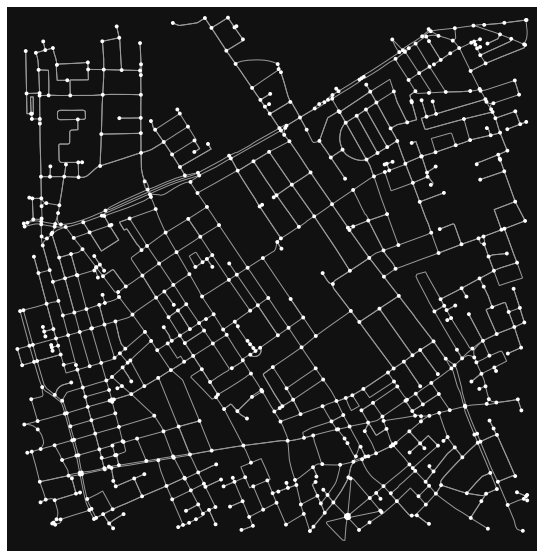
\includegraphics{./Figs/osmx1.png}
\end{frame}

\begin{frame}[fragile]{Vizato Rrjetin e Rrugës}
\protect\hypertarget{vizato-rrjetin-e-rruguxebs-4}{}
Skajet përmbajnë atribute, si emri i rrugës dhe lloji, të cilat mund të
aksesohen si një dataframe gjeografik.

python\AddToHookNext{env/Highlighting/begin}{\tiny}

\begin{Shaded}
\begin{Highlighting}[]
\CommentTok{\# Merrni vetëm skajet nga grafiku}
\NormalTok{edges\_df }\OperatorTok{=}\NormalTok{ osmnx.graph\_to\_gdfs(streets\_g, nodes}\OperatorTok{=}\VariableTok{False}\NormalTok{, edges}\OperatorTok{=}\VariableTok{True}\NormalTok{)}
\NormalTok{edges\_df.sample(}\DecValTok{3}\NormalTok{)}
\end{Highlighting}
\end{Shaded}
\end{frame}

\begin{frame}{Vizato Rrjetin e Rrugës}
\protect\hypertarget{vizato-rrjetin-e-rruguxebs-5}{}
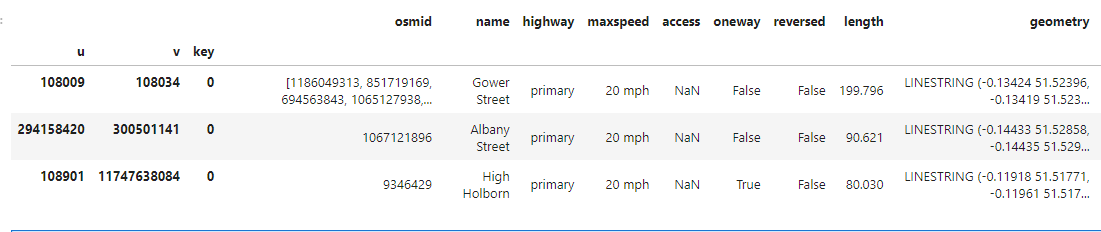
\includegraphics{./Figs/rrjetirrugor.png}
\end{frame}

\begin{frame}[fragile]{Vizato Rrjetin e Rrugës}
\protect\hypertarget{vizato-rrjetin-e-rruguxebs-6}{}
python\AddToHookNext{env/Highlighting/begin}{\tiny}

\begin{Shaded}
\begin{Highlighting}[]
\NormalTok{edges\_df.plot()}
\end{Highlighting}
\end{Shaded}
\end{frame}

\begin{frame}{Vizato Rrjetin e Rrugës}
\protect\hypertarget{vizato-rrjetin-e-rruguxebs-7}{}
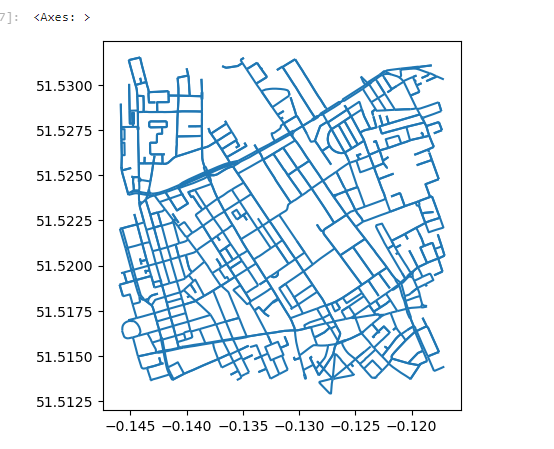
\includegraphics{./Figs/rrjetirrugor2.png}
\end{frame}

\begin{frame}[fragile]{Vizato Rrjetin e Rrugës}
\protect\hypertarget{vizato-rrjetin-e-rruguxebs-8}{}
Nyjet gjithashtu mund të kenë atribute, të tilla si vendndodhja dhe
numri i skajeve ndërprerëse:

python\AddToHookNext{env/Highlighting/begin}{\tiny}

\begin{Shaded}
\begin{Highlighting}[]
\CommentTok{\# Merrni nyjet nga grafiku si një kuadër të dhënash}
\NormalTok{nodes\_df }\OperatorTok{=}\NormalTok{ osmnx.graph\_to\_gdfs(streets\_g, nodes}\OperatorTok{=}\VariableTok{True}\NormalTok{, edges}\OperatorTok{=}\VariableTok{False}\NormalTok{)}
\NormalTok{nodes\_df.sample(}\DecValTok{5}\NormalTok{)}

\CommentTok{\# vizatoni nyjet}
\NormalTok{nodes\_df.plot()}
\end{Highlighting}
\end{Shaded}
\end{frame}

\begin{frame}{Vizato Rrjetin e Rrugës}
\protect\hypertarget{vizato-rrjetin-e-rruguxebs-9}{}
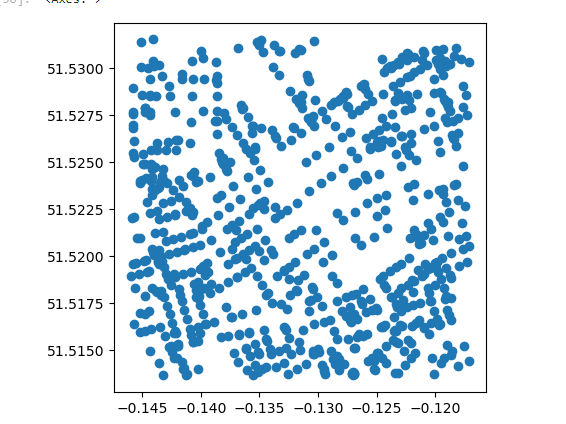
\includegraphics{./Figs/rrjetirrugor1.png}
\end{frame}

\begin{frame}[fragile]{Projekto Rrjetin}
\protect\hypertarget{projekto-rrjetin}{}
Për të punuar në rrjetet rrugore, është e nevojshme t'i projektoni ato
në një sistem të përshtatshëm të referencës koordinative.

python\AddToHookNext{env/Highlighting/begin}{\tiny}

\begin{Shaded}
\begin{Highlighting}[]
\BuiltInTok{print}\NormalTok{(}\StringTok{"Sistemi i koordinatave të nyjeve:"}\NormalTok{, nodes\_df.crs)}
\BuiltInTok{print}\NormalTok{(}\StringTok{"Sistemi i koordinatave të skajeve:"}\NormalTok{, edges\_df.crs)}
\end{Highlighting}
\end{Shaded}
\end{frame}

\begin{frame}{Projekto Rrjetin}
\protect\hypertarget{projekto-rrjetin-1}{}
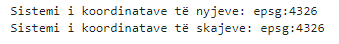
\includegraphics{./Figs/rrjetikor.png}
\end{frame}

\begin{frame}[fragile]{Projekto Rrjetin}
\protect\hypertarget{projekto-rrjetin-2}{}
Projektimi i këtij rrjeti rrugor në British National Grid:

python\AddToHookNext{env/Highlighting/begin}{\tiny}

\begin{Shaded}
\begin{Highlighting}[]
\NormalTok{streets\_g }\OperatorTok{=}\NormalTok{ osmnx.project\_graph(streets\_g, }\DecValTok{27700}\NormalTok{)}

\CommentTok{\# kontrolloni nëse projektimi funksionoi}
\NormalTok{nodes\_proj, edges\_proj }\OperatorTok{=}\NormalTok{ osmnx.graph\_to\_gdfs(streets\_g, nodes}\OperatorTok{=}\VariableTok{True}\NormalTok{, edges}\OperatorTok{=}\VariableTok{True}\NormalTok{)}
\BuiltInTok{print}\NormalTok{(nodes\_proj.crs)}
\BuiltInTok{print}\NormalTok{(edges\_proj.crs)}
\end{Highlighting}
\end{Shaded}
\end{frame}

\begin{frame}{Projekto Rrjetin}
\protect\hypertarget{projekto-rrjetin-3}{}
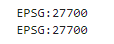
\includegraphics{./Figs/rrjetikor2.png}
\end{frame}

\begin{frame}[fragile]{Projekto Rrjetin}
\protect\hypertarget{projekto-rrjetin-4}{}
Tani koordinatat janë projektuar

python\AddToHookNext{env/Highlighting/begin}{\tiny}

\begin{Shaded}
\begin{Highlighting}[]
\NormalTok{edges\_proj.sample(}\DecValTok{5}\NormalTok{)}
\end{Highlighting}
\end{Shaded}
\end{frame}

\begin{frame}{Projekto Rrjetin}
\protect\hypertarget{projekto-rrjetin-5}{}
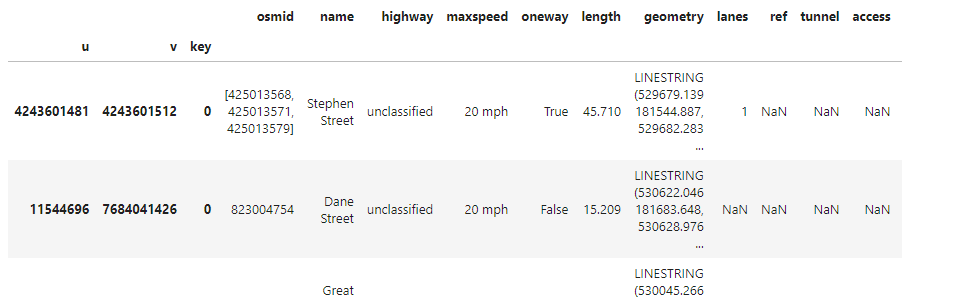
\includegraphics{./Figs/rrjetikor3.png}
\end{frame}

\begin{frame}[fragile]{Ndërtojmë përsëri}
\protect\hypertarget{nduxebrtojmuxeb-puxebrsuxebri}{}
python\AddToHookNext{env/Highlighting/begin}{\tiny}

\begin{Shaded}
\begin{Highlighting}[]
\NormalTok{osmnx.plot\_graph(streets\_g, figsize}\OperatorTok{=}\NormalTok{(}\DecValTok{10}\NormalTok{,}\DecValTok{10}\NormalTok{))}
\end{Highlighting}
\end{Shaded}
\end{frame}

\begin{frame}{Ndërtojmë përsëri}
\protect\hypertarget{nduxebrtojmuxeb-puxebrsuxebri-1}{}
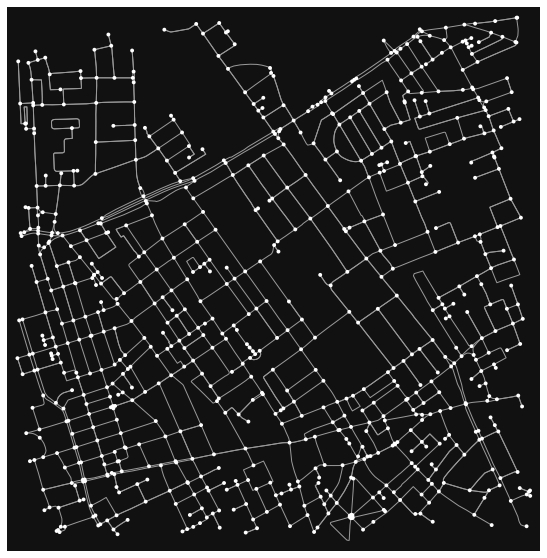
\includegraphics{./Figs/osmx3.png}
\end{frame}

\begin{frame}[fragile]{Analiza e Rrjetit}
\protect\hypertarget{analiza-e-rrjetit}{}
Rrjetet rrugore mund të analizohen në aspektin e strukturës së tyre
(morfologji) duke përdorur një sërë treguesish:

python\AddToHookNext{env/Highlighting/begin}{\tiny}

\begin{Shaded}
\begin{Highlighting}[]
\ImportTok{import}\NormalTok{ osmnx }\ImportTok{as}\NormalTok{ ox}

\CommentTok{\# Merrni statistikat bazike të rrjetit}
\NormalTok{basic\_stats }\OperatorTok{=}\NormalTok{ ox.basic\_stats(streets\_g)}
\NormalTok{basic\_stats}
\end{Highlighting}
\end{Shaded}
\end{frame}

\begin{frame}[fragile]{Llogaritja e Rrugëve}
\protect\hypertarget{llogaritja-e-rruguxebve}{}
Një pjesë qendrore në udhëzime është llogaritja e rrugëve më të shkurtra
në rrjetet rrugore.

python\AddToHookNext{env/Highlighting/begin}{\tiny}

\begin{Shaded}
\begin{Highlighting}[]
\ImportTok{import}\NormalTok{ random}
\ImportTok{import}\NormalTok{ networkx }\ImportTok{as}\NormalTok{ nx}
\ImportTok{import}\NormalTok{ matplotlib.pyplot }\ImportTok{as}\NormalTok{ plt}
\ImportTok{from}\NormalTok{ networkx.exception }\ImportTok{import}\NormalTok{ NetworkXNoPath}

\CommentTok{\# zgjidhni dy nyje të rastësishme}
\NormalTok{nodes }\OperatorTok{=}\NormalTok{ [n }\ControlFlowTok{for}\NormalTok{ n }\KeywordTok{in}\NormalTok{ streets\_g.nodes]}
\NormalTok{orig\_node }\OperatorTok{=}\NormalTok{ random.choice(nodes)}
\NormalTok{dest\_node }\OperatorTok{=}\NormalTok{ random.choice(nodes)}
\BuiltInTok{print}\NormalTok{(}\StringTok{"Nyja e origjinës:"}\NormalTok{, orig\_node, }\StringTok{", nyja e destinacionit:"}\NormalTok{, dest\_node)}
\end{Highlighting}
\end{Shaded}
\end{frame}

\begin{frame}[fragile]{Llogaritja e Rrugëve (vazhdim)}
\protect\hypertarget{llogaritja-e-rruguxebve-vazhdim}{}
python\AddToHookNext{env/Highlighting/begin}{\tiny}

\begin{Shaded}
\begin{Highlighting}[]
\CommentTok{\# Përpiquni/gjeni se për shkak se ndonjëherë rrugët nuk mund të gjenden}
\ControlFlowTok{try}\NormalTok{:}
    \CommentTok{\# gjeni rrugën më të shkurtër midis dy nyjeve}
\NormalTok{    route }\OperatorTok{=}\NormalTok{ nx.shortest\_path(streets\_g, orig\_node, dest\_node, weight}\OperatorTok{=}\StringTok{\textquotesingle{}length\textquotesingle{}}\NormalTok{)}
\NormalTok{    route\_len\_m }\OperatorTok{=}\NormalTok{ nx.shortest\_path\_length(streets\_g, orig\_node, dest\_node, weight}\OperatorTok{=}\StringTok{\textquotesingle{}length\textquotesingle{}}\NormalTok{)}
    \BuiltInTok{print}\NormalTok{(}\StringTok{"Rruga e udhëtimit e gjetur:"}\NormalTok{, }\BuiltInTok{len}\NormalTok{(route), }\StringTok{"segmente; gjatësi (m)"}\NormalTok{, }\BuiltInTok{round}\NormalTok{(route\_len\_m))}
    
    \CommentTok{\# vizatoni rrugën}
\NormalTok{    plt.figure(figsize}\OperatorTok{=}\NormalTok{(}\DecValTok{6}\NormalTok{, }\DecValTok{6}\NormalTok{))}
\NormalTok{    fig, ax }\OperatorTok{=}\NormalTok{ ox.plot\_graph\_route(streets\_g, route, route\_linewidth}\OperatorTok{=}\DecValTok{6}\NormalTok{, node\_size}\OperatorTok{=}\DecValTok{0}\NormalTok{, bgcolor}\OperatorTok{=}\StringTok{\textquotesingle{}k\textquotesingle{}}\NormalTok{)}
\ControlFlowTok{except}\NormalTok{ NetworkXNoPath }\ImportTok{as}\NormalTok{ e: }
    \BuiltInTok{print}\NormalTok{(}\StringTok{"Rruga nuk u gjet"}\NormalTok{, e)}
\end{Highlighting}
\end{Shaded}
\end{frame}

\begin{frame}{Llogaritja e Rrugëve}
\protect\hypertarget{llogaritja-e-rruguxebve-1}{}
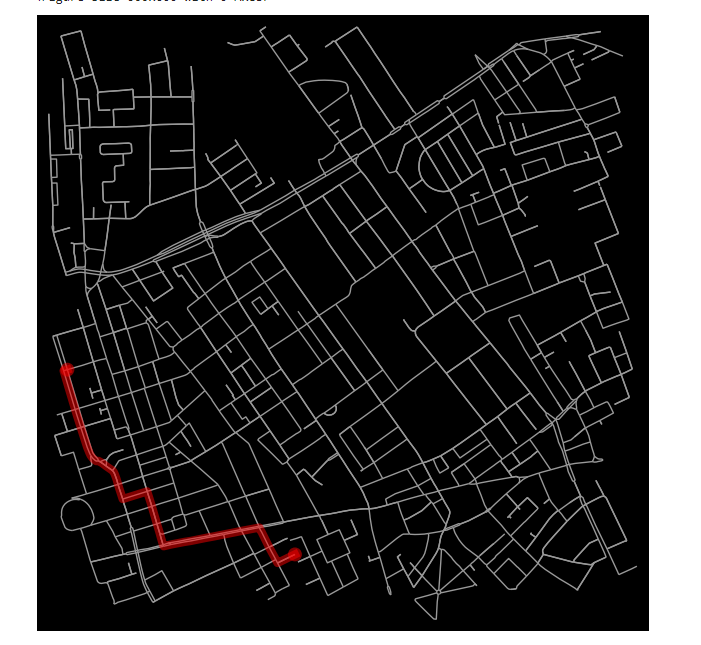
\includegraphics{./Figs/rrugshkurter.png}
\end{frame}

\begin{frame}[fragile]{Gjetja e Nyjeve Më të Afërta}
\protect\hypertarget{gjetja-e-nyjeve-muxeb-tuxeb-afuxebrta}{}
\begin{itemize}
\tightlist
\item
  Kur udhëtoni nga pika A në pikën B, hapi i parë është të gjeni nyjet
  më të afërta me A dhe B.
\end{itemize}

python\AddToHookNext{env/Highlighting/begin}{\tiny}

\begin{Shaded}
\begin{Highlighting}[]
\ImportTok{import}\NormalTok{ networkx }\ImportTok{as}\NormalTok{ nx}
\ImportTok{import}\NormalTok{ osmnx }\ImportTok{as}\NormalTok{ ox}

\CommentTok{\# Funksioni për të gjetur nyjen më të afërt}
\KeywordTok{def}\NormalTok{ get\_nearest\_node(graph, point):}
\NormalTok{    nearest\_node }\OperatorTok{=} \BuiltInTok{min}\NormalTok{(graph.nodes, key}\OperatorTok{=}\KeywordTok{lambda}\NormalTok{ n: ox.distance.great\_circle\_vec(point[}\DecValTok{1}\NormalTok{], point[}\DecValTok{0}\NormalTok{], graph.nodes[n][}\StringTok{\textquotesingle{}y\textquotesingle{}}\NormalTok{], graph.nodes[n][}\StringTok{\textquotesingle{}x\textquotesingle{}}\NormalTok{]))}
    \ControlFlowTok{return}\NormalTok{ nearest\_node}


\NormalTok{birkbeck\_node }\OperatorTok{=}\NormalTok{ get\_nearest\_node(streets\_g, birkbeck\_loc\_bg)}
\NormalTok{britishmus\_node }\OperatorTok{=}\NormalTok{ get\_nearest\_node(streets\_g, britishmus\_loc\_bg)}

\BuiltInTok{print}\NormalTok{(}\StringTok{"Nyjet më të afërta (ID{-}të):"}\NormalTok{, birkbeck\_node, britishmus\_node)}
\end{Highlighting}
\end{Shaded}
\end{frame}

\begin{frame}[fragile]{Llogaritja e Rrugës së Udhëtimit}
\protect\hypertarget{llogaritja-e-rruguxebs-suxeb-udhuxebtimit}{}
python\AddToHookNext{env/Highlighting/begin}{\tiny}

\begin{Shaded}
\begin{Highlighting}[]
\CommentTok{\# llogarisni rrugën e udhëtimit}
\NormalTok{route }\OperatorTok{=}\NormalTok{ nx.shortest\_path(streets\_g, birkbeck\_node, britishmus\_node, weight}\OperatorTok{=}\StringTok{\textquotesingle{}length\textquotesingle{}}\NormalTok{)}
\NormalTok{route\_len\_m }\OperatorTok{=}\NormalTok{ nx.shortest\_path\_length(streets\_g, orig\_node, dest\_node, weight}\OperatorTok{=}\StringTok{\textquotesingle{}length\textquotesingle{}}\NormalTok{)}
\BuiltInTok{print}\NormalTok{(}\StringTok{"Rruga midis Birkbeck dhe British Museum e gjetur:"}\NormalTok{, }\BuiltInTok{len}\NormalTok{(route), }\StringTok{"segmente; gjatësi (m)"}\NormalTok{, }\BuiltInTok{round}\NormalTok{(route\_len\_m))}
\end{Highlighting}
\end{Shaded}
\end{frame}

\begin{frame}[fragile]{vizatoni rrugën}
\protect\hypertarget{vizatoni-rruguxebn}{}
python\AddToHookNext{env/Highlighting/begin}{\tiny}

\begin{Shaded}
\begin{Highlighting}[]
\NormalTok{plt.figure(figsize}\OperatorTok{=}\NormalTok{(}\DecValTok{6}\NormalTok{, }\DecValTok{6}\NormalTok{))}
\NormalTok{fig, ax }\OperatorTok{=}\NormalTok{ ox.plot\_graph\_route(streets\_g, route, route\_linewidth}\OperatorTok{=}\DecValTok{6}\NormalTok{, node\_size}\OperatorTok{=}\DecValTok{0}\NormalTok{, bgcolor}\OperatorTok{=}\StringTok{\textquotesingle{}k\textquotesingle{}}\NormalTok{)}
\end{Highlighting}
\end{Shaded}

Këto të dhëna të rrjetit dhe mjetet mund të përdoren në një sërë
aplikimesh.
\end{frame}

\begin{frame}{vizatoni rrugën}
\protect\hypertarget{vizatoni-rruguxebn-1}{}
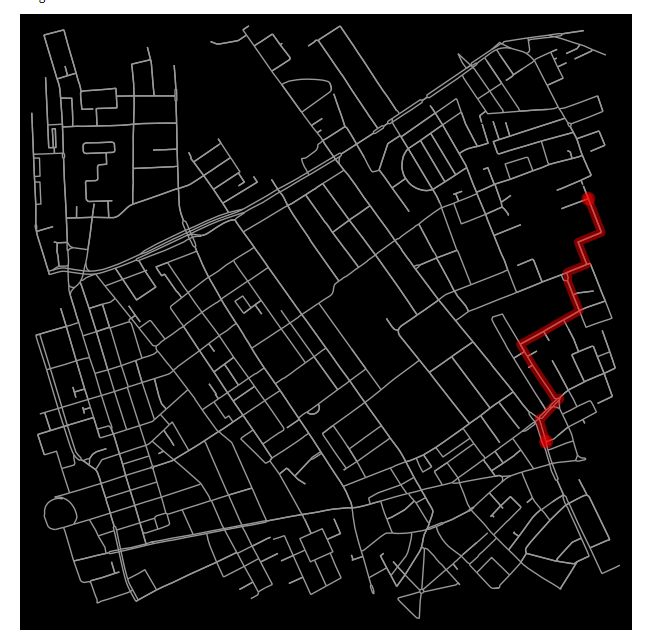
\includegraphics{./Figs/rrugshkurter2.png}
\end{frame}

\end{document}
